\documentclass[11pt, a4paper, logo, copyright, nonumbering]{SAI}
\usepackage[authoryear, sort&compress, round]{natbib}
\usepackage{dblfloatfix}
\usepackage{ulem}
\usepackage{caption}
\usepackage{dramatist}
\usepackage{xspace}
\usepackage{pifont} %
\usepackage{multirow}
\usepackage{tcolorbox}
\usepackage{xltabular}
\usepackage{longtable}
\usepackage{hyperref}
\interfootnotelinepenalty=10000

\usepackage{amsfonts}
\usepackage{amsmath}
\usepackage{amssymb}
\usepackage{lineno}
\usepackage{multirow}
\usepackage{adjustbox}

\usepackage[bottom]{footmisc}

\usepackage{CJKutf8}
\usepackage{subfigure}
\usepackage{setspace}

\usepackage{dsfont}
\usepackage{array} %
\usepackage{tabularx} %
\usepackage{subfigure} %
\usepackage{xcolor} %
\usepackage{tabularx}
\usepackage{booktabs}

\usepackage{lipsum}  %
\usepackage{multicol} %




\makeatletter
\def\@BTrule[#1]{%
  \ifx\longtable\undefined
    \let\@BTswitch\@BTnormal
  \else\ifx\hline\LT@hline
    \nobreak
    \let\@BTswitch\@BLTrule
  \else
     \let\@BTswitch\@BTnormal
  \fi\fi
  \global\@thisrulewidth=#1\relax
  \ifnum\@thisruleclass=\tw@\vskip\@aboverulesep\else
  \ifnum\@lastruleclass=\z@\vskip\@aboverulesep\else
  \ifnum\@lastruleclass=\@ne\vskip\doublerulesep\fi\fi\fi
  \@BTswitch}
\makeatother

\addto\extrasenglish{
    \def\chapterautorefname{Chapter}%
    \def\sectionautorefname{Section}%
    \def\paragraphautorefname{Section}
    \def\subparagraphautorefname{Section}
    \def\paragraphautorefname{Paragraph}%
    \def\tableautorefname{Table}%
    \def\equationautorefname{Equation}%
}

\newenvironment{indentchunk}[1]%
 {\begin{list}{}%
         {\setlength{\leftmargin}{#1}}%
         \item[]%
 }
 {\end{list}}
 
\bibliographystyle{abbrvnat}

\reportnumber{001} %


\title{\textsc{PhysMaster}: Building an Autonomous AI Physicist \\for Theoretical and Computational Physics Research}

\author{
    Tingjia Miao\textsuperscript{\rm 1,2,5} \quad
    Jiawen Dai\textsuperscript{\rm 2} \quad
    Jingkun Liu\textsuperscript{\rm 2} \quad 
    Jinxin Tan\textsuperscript{\rm 2,3,4} \quad 
    Muhua Zhang\textsuperscript{\rm 2,3,4} \quad
    Wenkai Jin\textsuperscript{\rm 1} \quad     
    Yuwen Du\textsuperscript{\rm 1} \quad 
    Tian Jin\textsuperscript{\rm 1} \quad 
    Xianghe Pang\textsuperscript{\rm 1} \quad 
    Zexi Liu\textsuperscript{\rm 1} \quad 
    Tu Guo\textsuperscript{\rm 2,4}  \quad
    Zhengliang Zhang \textsuperscript{\rm 2,4,5} \quad
    Yunjie Huang\textsuperscript{\rm 1} \quad 
    Shuo Chen\textsuperscript{\rm 6} \quad
    Rui Ye\textsuperscript{\rm 1} \quad 
    Yuzhi Zhang\textsuperscript{\rm 7} \quad
    Linfeng Zhang\textsuperscript{\rm 7} \quad 
    Kun Chen\textsuperscript{\rm 6} \quad \quad \quad
    Wei Wang\textsuperscript{\rm 2,3,4} \quad
    Weinan E\textsuperscript{\rm 1} \quad
    Siheng Chen\textsuperscript{\rm 1}
    \\
    \textsuperscript{\rm 1} School of Artificial Intelligence, Shanghai Jiao Tong University \quad \\
    \textsuperscript{\rm 2} School of Physics and Astronomy, Shanghai Jiao Tong University \quad \\
    \textsuperscript{\rm 3} State Key Laboratory of Dark Matter Physics, Shanghai Jiao Tong University  \quad \\
    \textsuperscript{\rm 4} Tsung-Dao Lee Institute, Shanghai Jiao Tong University\quad \\
    \textsuperscript{\rm 5} Zhiyuan College, Shanghai Jiao Tong University\quad  \\
    \textsuperscript{\rm 6} Institute of Theoretical Physics, Chinese Academy of Sciences \quad \textsuperscript{\rm 7} DP Technology
    }



\newcommand{\agent}{\textsc{PhysMaster}\xspace}
\newcommand{\knowledge}{\textsc{LANDAU}\xspace}
\newcommand{\xmark}{\textcolor{red}{\ensuremath{\times}}}
\newcommand{\cmark}{\textcolor[rgb]{0,0.51,0}{\checkmark}}
\newcommand{\ave}[1]{\left\langle #1 \right\rangle}
\newcommand{\op}[1]{\hat{#1}}
\newcommand{\dagop}[1]{\op{#1}^\dagger}

\begin{abstract}

Advances in AI have produced agents whose knowledge and operational capabilities are comparable to those of human scientists, revealing their potential to assist, accelerate, and automate scientific research, thereby fundamentally reshaping the paradigm of scientific discovery. However, prior works either evaluate models on well-defined benchmarks, such as Olympiad problems (e.g., IMO, IPhO) or factual question answering, or focus on general-purpose tasks such as literature retrieval and information integration, rather than end-to-end problem solving in open-ended scientific scenarios. As a result, AI remains inferior and auxiliary in real-world scientific research. In particular, in physics, a fundamental yet abstract, inherently complex, and intellectually demanding domain, research often requires both intensive analytical reasoning and code-based numerical computation, a dual capability largely absent in previous agents.

To meet the demands of physics research, we propose \agent, an LLM-based agent designed to operate as \emph{an autonomous theoretical and computational physicist}. \agent integrates theoretical reasoning and numerical computation techniques, and is further equipped with \knowledge, the \emph{Layered Academic DAta Universe} that preserves precise retrieved papers, manually curated prior knowledge and validated methodology traces for reuse to enhance decision reliability and stability. Further, an adaptive exploration methodology is applied to balance exploration with efficiency, and adapt to ultra-long-horizon tasks.

Spanning the scale from the cosmos to elementary particles, \agent has reliable capabilities across various subfields of theoretical physics, including high-energy theory, condensed matter theory, cosmology \& astrophysics, and quantum information, as validated by:

\vspace{-0.3ex}
\par\noindent\textbullet\xspace Two typical \emph{acceleration} cases, in which \agent compresses the labor-intensive engineering parts of genuine physics research into less than 6 hours, which typically requires 1-3 months of a senior Ph.D.;
\vspace{-0.3ex}
\par\noindent\textbullet\xspace Two \emph{automation} cases, in which the \agent is provided with a human-specified hypothesis or selected methods and automatically execute the exploration loop, conducting experiments, validating hypotheses, thereby compressing the end-to-end loop into 1 day, whereas the timeline is rather unpredictable and could take up months.
\vspace{-0.3ex}
\par\noindent\textbullet\xspace One \emph{autonomous discovery} case, where the agent conducts fully independent exploration of a scientific problem that remains open and proposes an innovative method, marking the transition from AI co-scientist to autonomous AI scientist.

From acceleration and automation to autonomous discovery, our work reveals the potential of AI in fundamental science and contributes to further AI-driven scientific discovery.

\end{abstract}

\begin{document}

\maketitle

\newpage

\begin{spacing}{0.9}
\tableofcontents
\end{spacing}

\newpage

\section{Introduction}
\label{sec:introduction}

\subsection{From Large Language Models (LLMs) to Agentic Intelligence}

The advancement in Large Language Models (LLMs) has profoundly reshaped both the ways we live and work, marking a new era in Artificial Intelligence (AI). From early conversational systems such as ChatGPT to more recent models~\cite{openai2024gpt4,jaech2024openai,guo2025deepseek}, LLMs have exhibited substantial gains in abstract reasoning, long-horizon planning, and multi-step problem-solving. When augmented with tool-use and action-taking capabilities~\cite{schmidgall2025agent}, these systems increasingly blur the boundary between passive language understanding and active task execution, raising the prospect that AI systems may approach---or in narrowly defined domains, surpass---human expert-level performance. 

This aligns with the staged framework for Artificial General Intelligence (AGI) articulated by OpenAI~\cite{openai2024agi}, which conceptualizes AI capabilities as several levels:

\vspace{-2.0ex}
\begin{itemize}
    \item \textbf{Level 1 — Chatbots:} AI with conversational language.
    \item \textbf{Level 2 — Reasoners:} human-level problem-solving.
    \item \textbf{Level 3 — Agents:} systems that can take actions.
    \item \textbf{Level 4 — Innovators:} AI that can aid in invention.
    \item \textbf{Level 5 — Organizations:} AI that can do the work of an orgnization.
\end{itemize}
\vspace{-2.0ex}

Current frontier systems, augmented with tool-use, planning, and execution capabilities, are believed to be at Level 3, which is Agents. Meanwhile, the transition from agentic execution (Level 3) to genuine innovation (Level 4) is accelerating, where AI systems can autonomously generate novel hypotheses, conduct verification and yield novel discoveries. Consequently, the human-AI collaboration paradigm will be fundamentally reshaped: \emph{from human-directed AI assistance towards AI-orchestrated task execution with human oversight, and ultimately to greater autonomy}.

\subsection{AI for Science and AI Scientist: From Tools to Autonomous Discovery}

It is widely recognized that AI holds the potential to \emph{transform scientific research paradigms and accelerate discoveries}. In earlier stages, AI primarily functioned as a powerful, tool-like enabler of science, supporting tasks such as prediction, simulation, and data-driven inference. Scientific foundation models have emerged as powerful capability engines, with recent domain-specific models setting or approaching frontiers in key sub-tasks. For instance, AlphaFold3 advances biomolecular structure and interaction prediction~\cite{abramson2024alphafold3}, while GNoME enables large-scale discovery of stable inorganic crystals~\cite{merchant2023gnome}. GraphCast demonstrates that learned surrogates can rival numerical simulators for complex dynamical systems with significant speedups~\cite{lam2023graphcast}, and Uni-Mol provides a universal 3D molecular representation framework unifying diverse downstream tasks~\cite{zhou2023unimol}. These breakthroughs furnish strong engines for inference, generation, and simulation—essential components of scientific cycles—yet they underscore that models alone address only fragments of scientific work and become transformative when integrated into larger systems.

As AI general capabilities advance, AI is evolving from a mere scientific tool to an active research labor force, enabling the rise of AI scientists that can autonomously participate in research and facilitate discovery, though within engineered environments. The AI co-scientist from Google/DeepMind, a multi-agent Gemini-based system, employs generate-debate-evolve cycles to propose biomedical hypotheses, some validated experimentally, while amplifying human scientists in prioritization and leaving final judgment to them~\cite{natarajan2025aicoscientist}. In parallel, The AI Scientist and AI Scientist-v2 from Sakana AI automate the research loop in machine learning—from ideation to experiment design and paper writing—achieving peer-reviewed acceptance of fully AI-generated papers~\cite{lu2024aiscientist,yamada2025aiscientistv2}. Beyond these, Robin offers a multi-agent framework automating literature research, hypothesis generation, experiment planning, and data analysis, applied in lab-in-the-loop settings to discover therapeutic candidates~\cite{ghareeb2025robin}. Further, the recent Kosmos sustaining long-horizon cycles of literature search, data analysis, and hypothesis generation to produce traceable scientific reports and cross-domain discoveries~\cite{mitchener2025kosmos}. Denario presents a modular multi-agent research assistant that covers idea generation, literature review, planning, and code execution across multiple scientific domains; however, the authors also reports frequent computational mistakes and occasional unsupported claims, underscoring the continued need for rigorous mathematical/numerical verification ~\cite{villaescusa2025denario}. Despite these impressive demonstrations, current AI scientist systems are still largely optimized for \emph{text-centric domains}, with limited ability to \emph{manipulate rigorous mathematical formalisms} and to \emph{conduct robust numerical computation} for verification, while also lacking the \emph{adaptability to long-horizon workflows}.

\subsection{\agent, the Autonomous AI Physicist}

Physics is a uniquely fundamental and comprehensive enterprise: it seeks universal principles spanning scales from the 
cosmos~\citep{peebles2020principles} to the micro quantum world where Quantum Chromodynamics (QCD) governs quarks and gluons~\citep{marciano1978quantum}.
Its unification comes from structures such as symmetry and gauge principles~\citep{noether1983invariante,yang1954conservation}, effective field theory~\citep{weinberg1979phenomenological}, and renormalization-group flow~\citep{wilson1975renormalization}, which systematically connect microscopic laws to macroscopic universality.
At the research frontier, these ideas are expressed in highly abstract formalism. For instance, Lie groups and representation theory~\citep{georgi2000lie}, differential geometry of gauge fields~\citep{wu1975concept}, and topology/anomaly constraints~\citep{adler1969axial} that rigidly delimit what theories are possible.
Meanwhile, state-of-the-art numerical methods (e.g., Quantum Monte Carlo, DMRG) is essential for quantitatively validating the proposed theories.
Therefore, physics stands as a monument to human intellect, shaped by generations of talented physicists who devoted their passion and wisdom, from Newton, Maxwell to Einstein, Landau, T.-D. Lee and C.-N. Yang. 
If AI can be integrated into physics research, it will \emph{liberate the talented from tedious engineering tasks and repetitive computations, accelerate the emergence of inspiration and its validation, and thereby help establish a new human–machine collaborative research paradigm}.

\vspace{-0.2ex}

Existing AI-for-physics efforts have achieved striking results but largely within \emph{isolated} slices of the research loop.
AI Feynman demonstrates physics-inspired symbolic regression that can recover compact closed-form relations from data~\cite{udrescu2020aifeynman}, yet it does not autonomously perform the broader workflow of choosing formalisms, managing approximations, and closing the loop with numerical verification and uncertainty control.
Physics-Informed Neural Networks (PINNs) incorporate PDE constraints into learning and can serve as flexible surrogates~\cite{raissi2019pinn}, but they typically presuppose a fixed modeling setup and often require expert tuning to remain reliable in stiff, multiscale, or long-time regimes---again falling short of end-to-end theory--computation iteration.
In quantum many-body physics, neural quantum states provide expressive variational wavefunction representations~\cite{carleo2017nqs}, but they still rely on expert-specified Hamiltonians and sampling/optimization protocols, rather than perform an end-to-end research loop.

\vspace{-0.2ex}

To meet the demands of physics research, we propose \agent, an LLM-based agent designed to operate as an autonomous theoretical and computational physicist. \agent integrates theoretical reasoning and numerical computation techniques, and is further equipped with a \emph{Layered Academic DAta Universe} (\textsc{LANDAU}), that preserves \emph{precisely retrieved papers, manually curated prior knowledge and validated methodology traces} for future reuse, enhancing both efficiency and decision stability. Further, an adaptive multi-trajectory exploration methodology is applied to balance exploration with efficiency, and \emph{adapt to ultra-long-horizon tasks}.

\begin{figure}[ht]
\centering
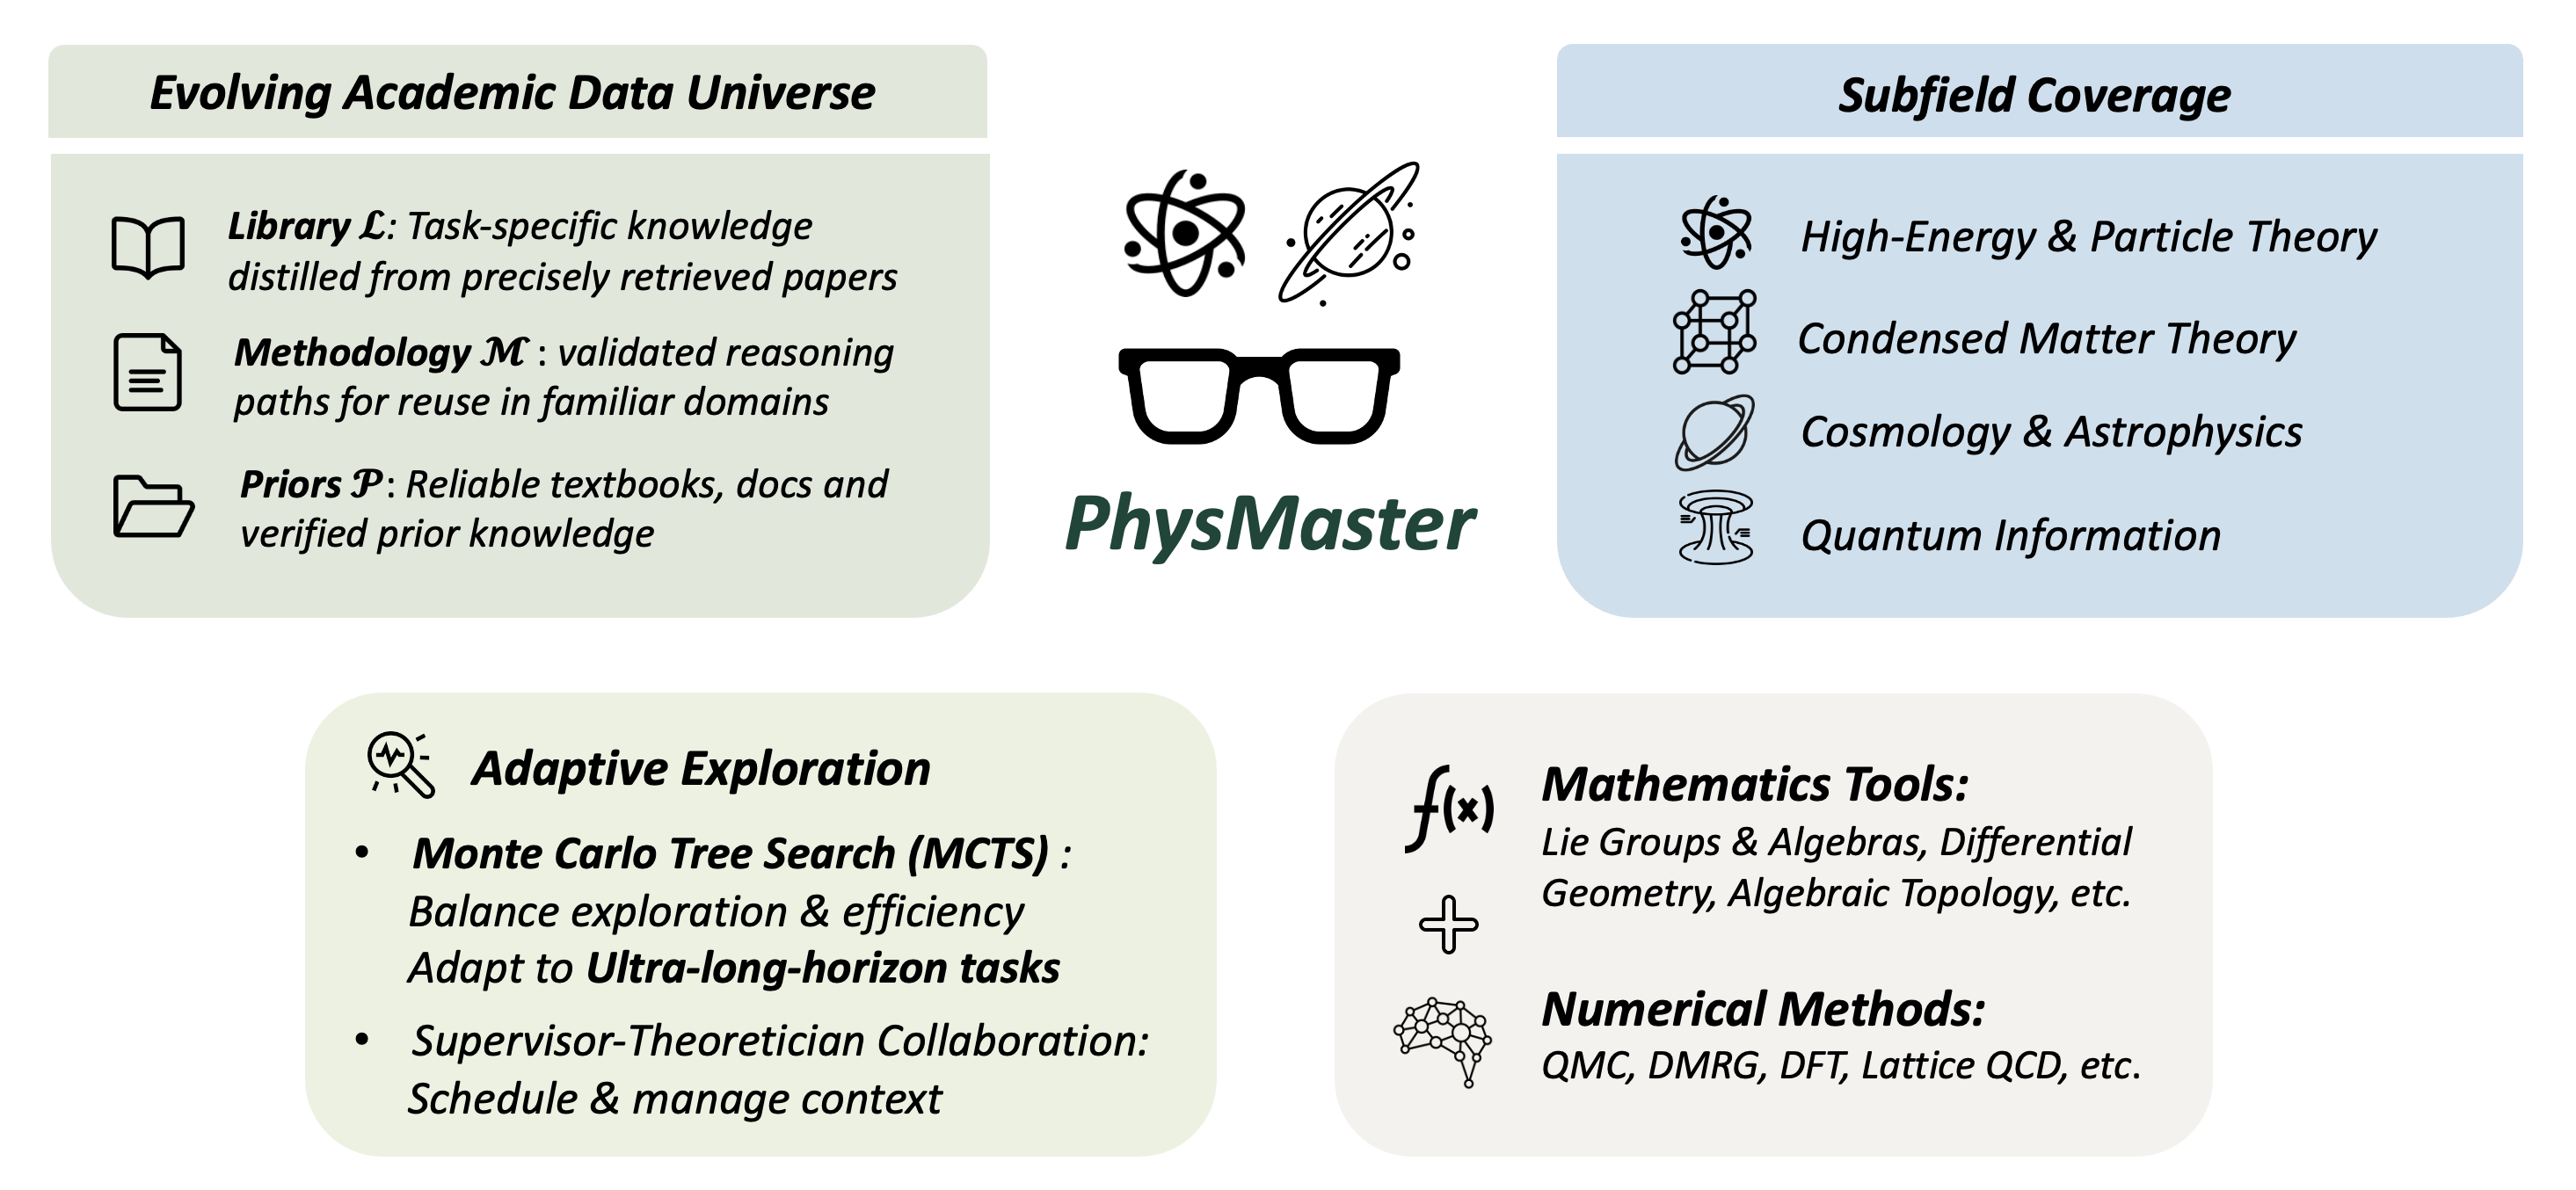
\includegraphics[width=0.9 \textwidth]{figure/overview.jpg}
\caption{The Core Features of \agent} 
\label{fig:core}
\end{figure}

Our system demonstrates state-of-the-art performance across diverse  mathematics \& code intensive physics subfields of theoretical \& computational physics, including but not limited to:

\vspace{-1.6ex}
\begin{enumerate}
    \item \textbf{High-Energy \& Particle Theory}: Quantum Field Theory \& Formal Theory (Yang–Mills theory, EFT, QCD and Strong coupling problems), Particle Physics Phenomenology, etc.
    \item \textbf{Condensed Matter Theory}: Many-Body Theory, Topological \& Quantum Phases (Topological Insulators \& Superconductors, Quantum Hall effect), Computational Condensed Matter (First-principles computation, Quantum Monte Carlo, Tensor-network), etc.
    \item \textbf{Cosmology \& Astrophysics}: Early Universe \& Inflation, Large-Scale Structure, Astroparticle Physics, Black Hole \& Gravity Theory, etc.
    \item \textbf{Quantum Information}: Quantum Information Theory, Quantum Computing Theory, etc.
\end{enumerate}
\vspace{-1.6ex}

While mainstream LLMs primarily excel at text generation and prone to unverified derivations or computational hallucinations, \agent provides: 

\vspace{-1.6ex}
\begin{enumerate}
    \item Ultra-long-horizon workflows via MCTS exploration with traceable trajectory
    \item Executable coding environments for feedbacks and self-evolution.
    \item The \knowledge preserves manually curated prior knowledge and validated methodology traces for reuse and retrieval-augmented generation (RAG) to enhance reliability.
\end{enumerate}
\vspace{-1.6ex}

In contrast to prior AI scientist prototypes, which operate effectively in stage-specific or domain-specific pipelines (e.g., literature-driven hypothesis generation or ML research automation), \agent is tailored to physics research by: 

\vspace{-1.6ex}
\begin{enumerate}
    \item Adopting a physicist mindset co-designed with domain experts
    \item Possessing the dual capability of rigorous theoretical reasoning and executable coding
    \item Leveraging an evolving physics-oriented knowledge base
    \item Autonomously executing an end-to-end, ultra-long-horizon research loop rather than being confined to a single stage
\end{enumerate}
\vspace{-1.6ex}

By bridging theoretical insight with computational prowess, \agent not only automates routine tasks but also fosters novel discoveries, paving the way for AI-led revolutions in physics research.

\newpage
\section{Architecture and Workflow}
We establish a phased multi-agent system (MAS) that solve problems via sequential collaboration, in which the workflow can be divided into three major phases: Pre-Task, Task Execution, and Post-Task. 

\begin{figure}[ht]
    \centering
    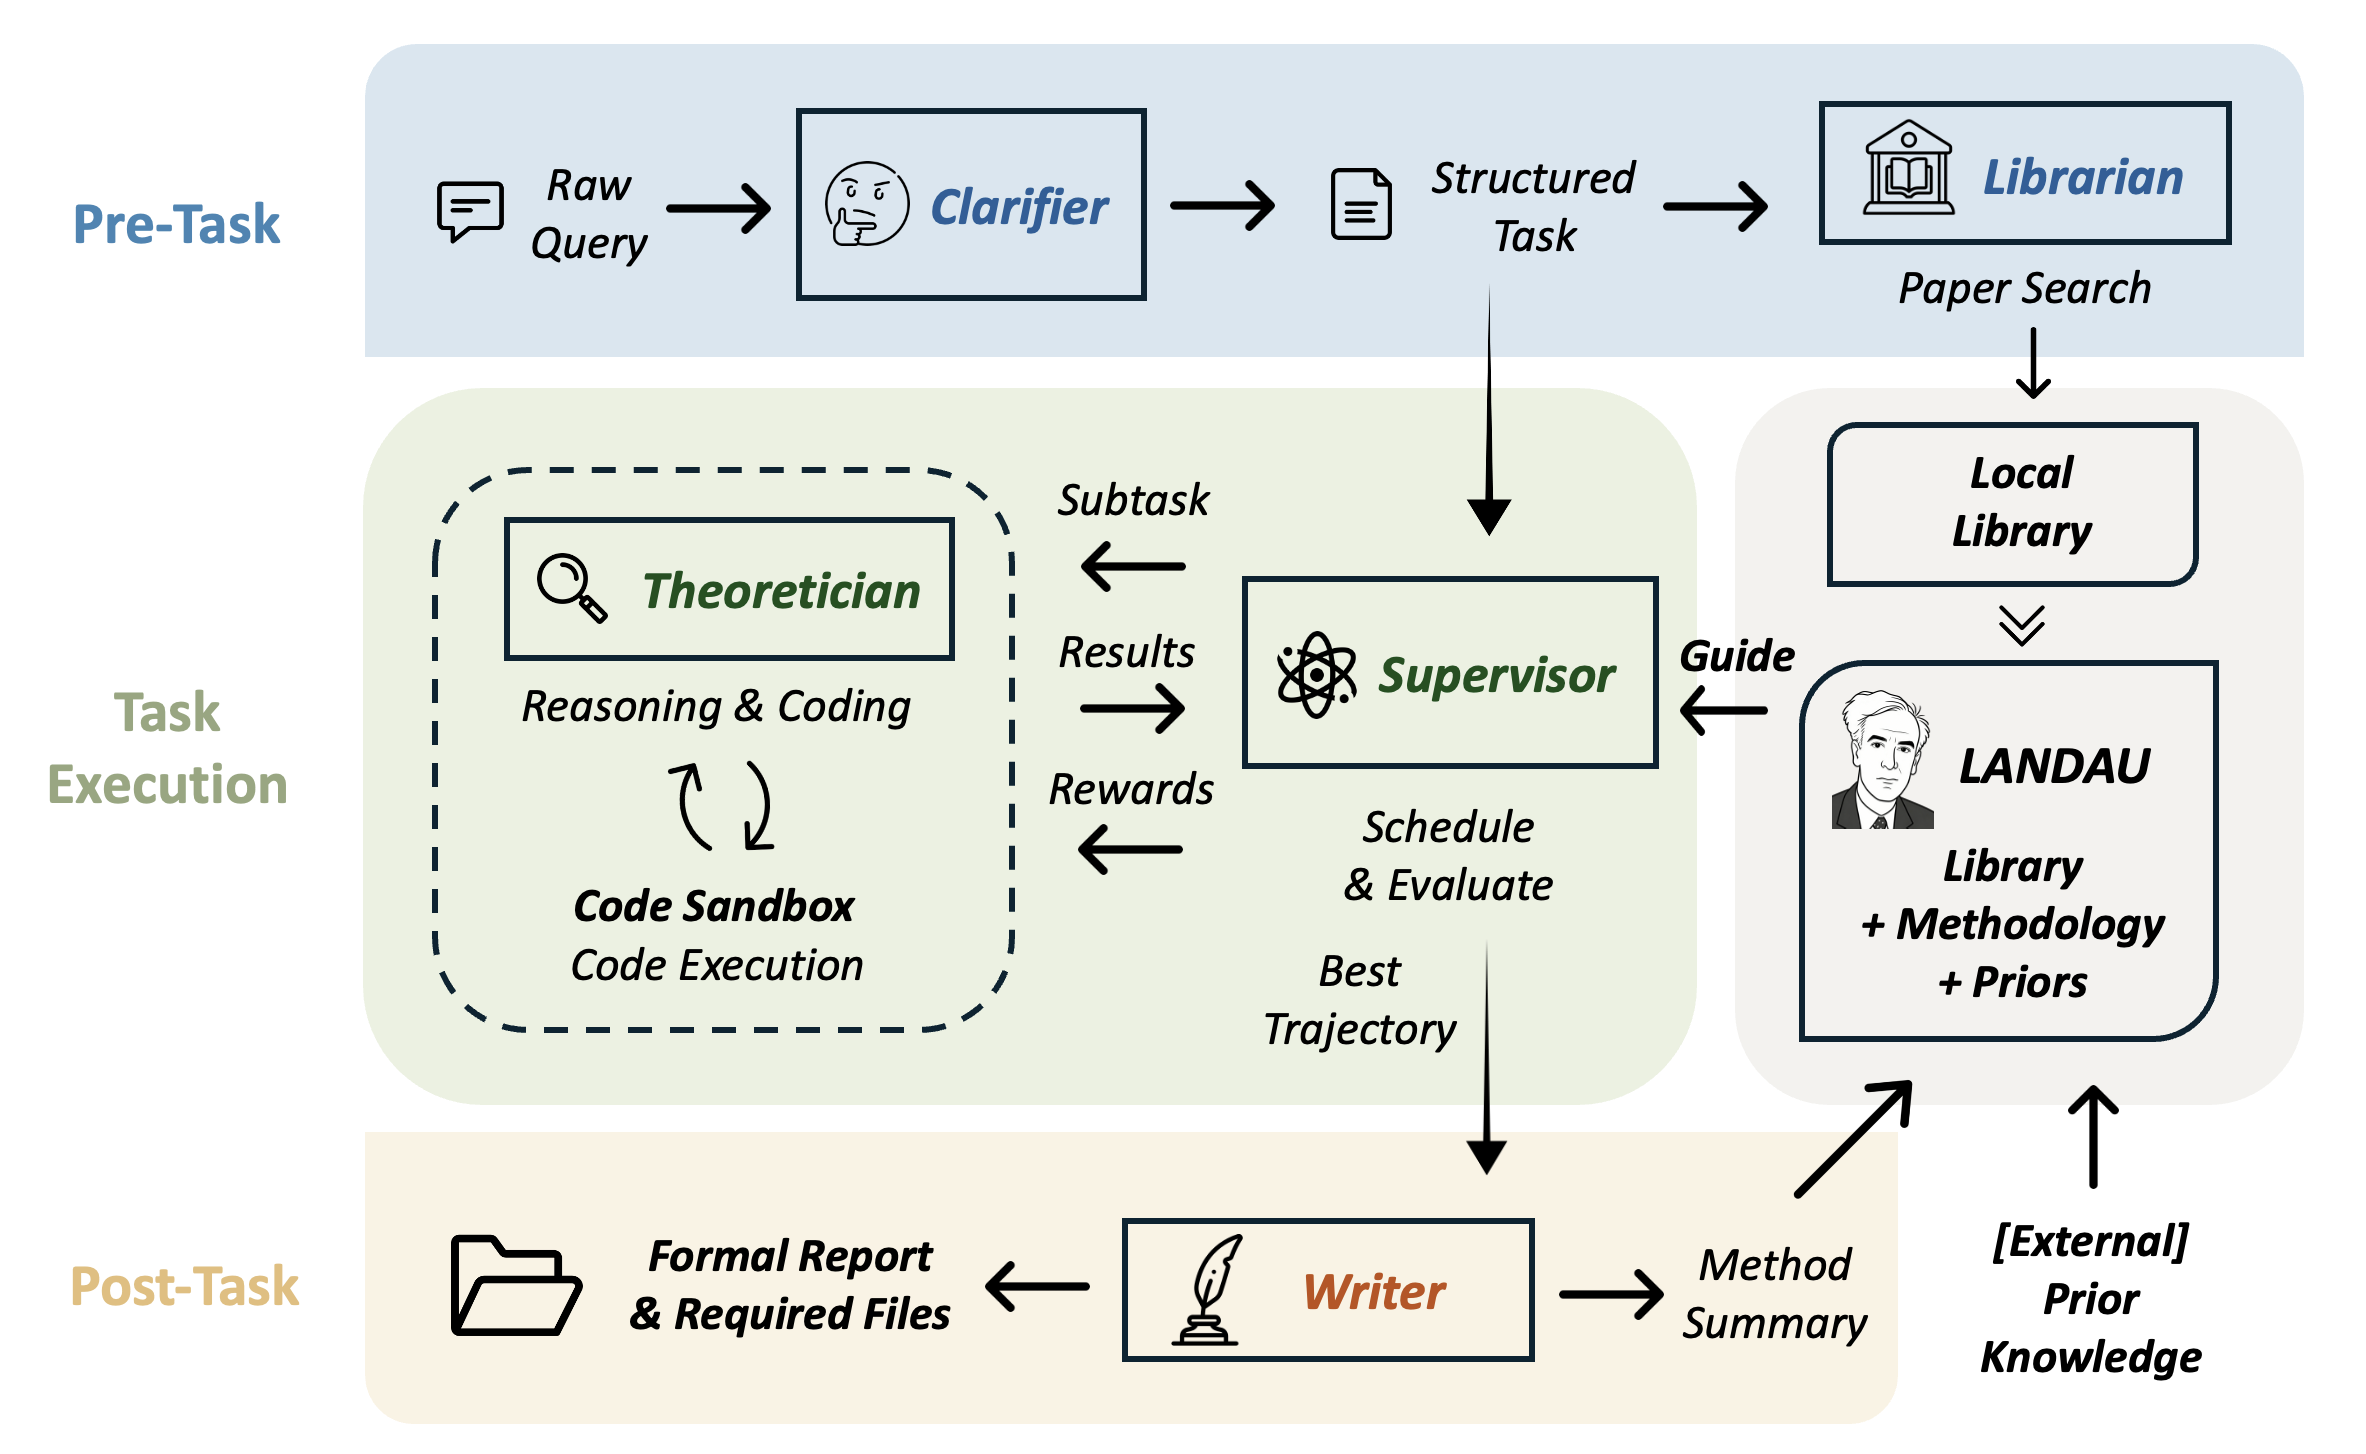
\includegraphics[width=0.8\linewidth]{figure/workflow.jpg}
    \caption{The MAS Architechture and Workflow of \agent}
    \label{fig:workflow}
\end{figure}

Our system adopts the mindset of physicists and integrate theoretical reasoning with code execution, thereby closing the loop from natural-language queries to research report with scientific rigor.

\subsection{Pre-Task: Query Clarification and Ultra-long-horizon Task Decomposition}
As the initial stage of the workflow, a Clarifier transforms the original natural-language query into a structured task by extracting essential information and decomposing it into subtasks.

The primary goal of this stage is to refine natural-language questions that tend to be information-heavy, lack semantic hierarchy, or contain ambiguities. This prevents structural redundancy and semantic ambiguity from inflating the token budget, obscuring key details, or even causing misunderstandings that lead the reasoning trajectory away from the intended problem. This process effectively improves both efficiency and efficacy, while sparing users from the burden of manually reorganizing queries into detailed, rigid formats. Conceptually, this stage also emulates how physicists in real research construct physical intuition---that is, by extracting simplified, intuitive, and abstract physical processes.

During this phase, the following information is extracted from the query:

\begin{itemize}
    \item \textbf{Basic information:} topic, domain, task description, Input and output formats, etc.
    \item \textbf{Task type:}
    \begin{itemize}
        \item \emph{Engineering Computation}: well-established models and mature methods requiring high-precision solutions, such as first-principles calculations or many-body numerics.
        \item \emph{Hypothesis Testing}: semi-open tasks that follow human-provided ideas or selected methodologies to attempt solving a problem or testing a hypothesis, involving a certain degree of innovation.
        \item \emph{Open-ended Exploration}: fully open tasks lacking a predefined framework or mechanism, requiring autonomous hypothesis formation and validation.
        \item \emph{Phenomenological Analysis}: bridging theory and experiment by extracting parameters from data, constructing effective parametrizations, fitting models, etc.
    \end{itemize}
    \item \textbf{Physical constraints:} symmetries, conservation laws, dimensional analysis, spacetime and energy scales, etc.
    \item \textbf{Relevant knowledge} for literature retrieval and knowledge-base construction.
    \item \textbf{Sequence of subtasks} for dynamic scheduling during Task Execution.
\end{itemize}


\subsection{Pre-Task: Literature Precise Retrieval and Local Library Construction}

Building upon our previous work \textsc{Paper Search Master}, a comprehensive academic paper search agent, we develop a physics-oriented literature retrieval module that constructs a task-specific local library $\mathcal{L}_{Local}$. To ensure coverage, depth, and reliability, the retrieval process is jointly driven by two complementary agents:

\begin{itemize}
    \item \textbf{Quick Thinker}: Operates based on intuition-driven expansion. It searches directly from queries or extends from retrieved papers using multiple retrieval tools, rapidly forming a broad candidate pool.
    \item \textbf{Reasoner}: Utilizes strong reasoning capabilities to understand the problem context deeply and filter out papers with high semantic relevance to the query.
\end{itemize}

For each piece relevant knowledge extracted during the clarification, a precise retrieval round is executed. From each highly-relevant paper, we extract two categories of knowledge:

\begin{itemize}
    \item \textbf{Qualitative Knowledge}: Physical principles, mechanisms, and conceptual structures (e.g., the existence of a phase transition, dominant competing effects). These guide the task-execution agent to grasp essential physics and avoid foundational errors.
    \item \textbf{Quantitative Knowledge}: Analytical expressions, precise numerical results, or calibrated parameters that support model construction and numerical computation, forming the basis for reliable criticism.
\end{itemize}

This task-specific local library $\mathcal{L}_{Local}$ serves as the foundation for retrieval-augmented generation (RAG) in the Task Execution stage. The integration of qualitative and quantitative knowledge enables the system to overcome hallucination and shift from language generation to evidence-grounded scientific reasoning. The benefits of $\mathcal{L}_{Local}$ are summarized as follows:

\begin{itemize}
    \item \textbf{Traceability}: Each RAG decision is interpretable and verifiable via evidence chain.
    \item \textbf{Generalization}: Task-specific construction of $\mathcal{L}_{Local}$ enables rapid adaptation to new research directions (e.g., quantum many-body, condensed matter, high-energy physics) without additional fine-tuning.
    \item \textbf{Long-Context Integration}: Physics research often spans multiple papers, decades of theoretical development, and methodological comparisons. Through retrieval--filtering--reconstruction, RAG allows LLMs to operate on knowledge far exceeding their native context window in a structured and efficient manner.
\end{itemize}


\subsection{Task Execution: MCTS and Hierarchical Agent Collaboration}
Solving real scientific problems in theoretical or computational physics is typically an ultra-long-horizon test-time scaling task, often requiring proper task decomposition, flexible subtask scheduling, and a large number of iterations of draft--evaluate--revise that exceed the context window of any single model. Therefore, context management becomes the core systems challenge, meaning that the agent must preserve progress and reuse experience without accumulating an ever-growing prompt.

Inspired by ML-Master~\cite{liu2025ml}, we adopt Monte Carlo Tree Search (MCTS) to balance exploration and efficiency when dealing with such tasks. In essence, each MCTS node represents an attempt to search for or refine a partial solution. Through multi-trajectory expansion, the process ultimately yields an optimal trajectory that serves as the complete solution.

\begin{figure}[ht]
    \centering
    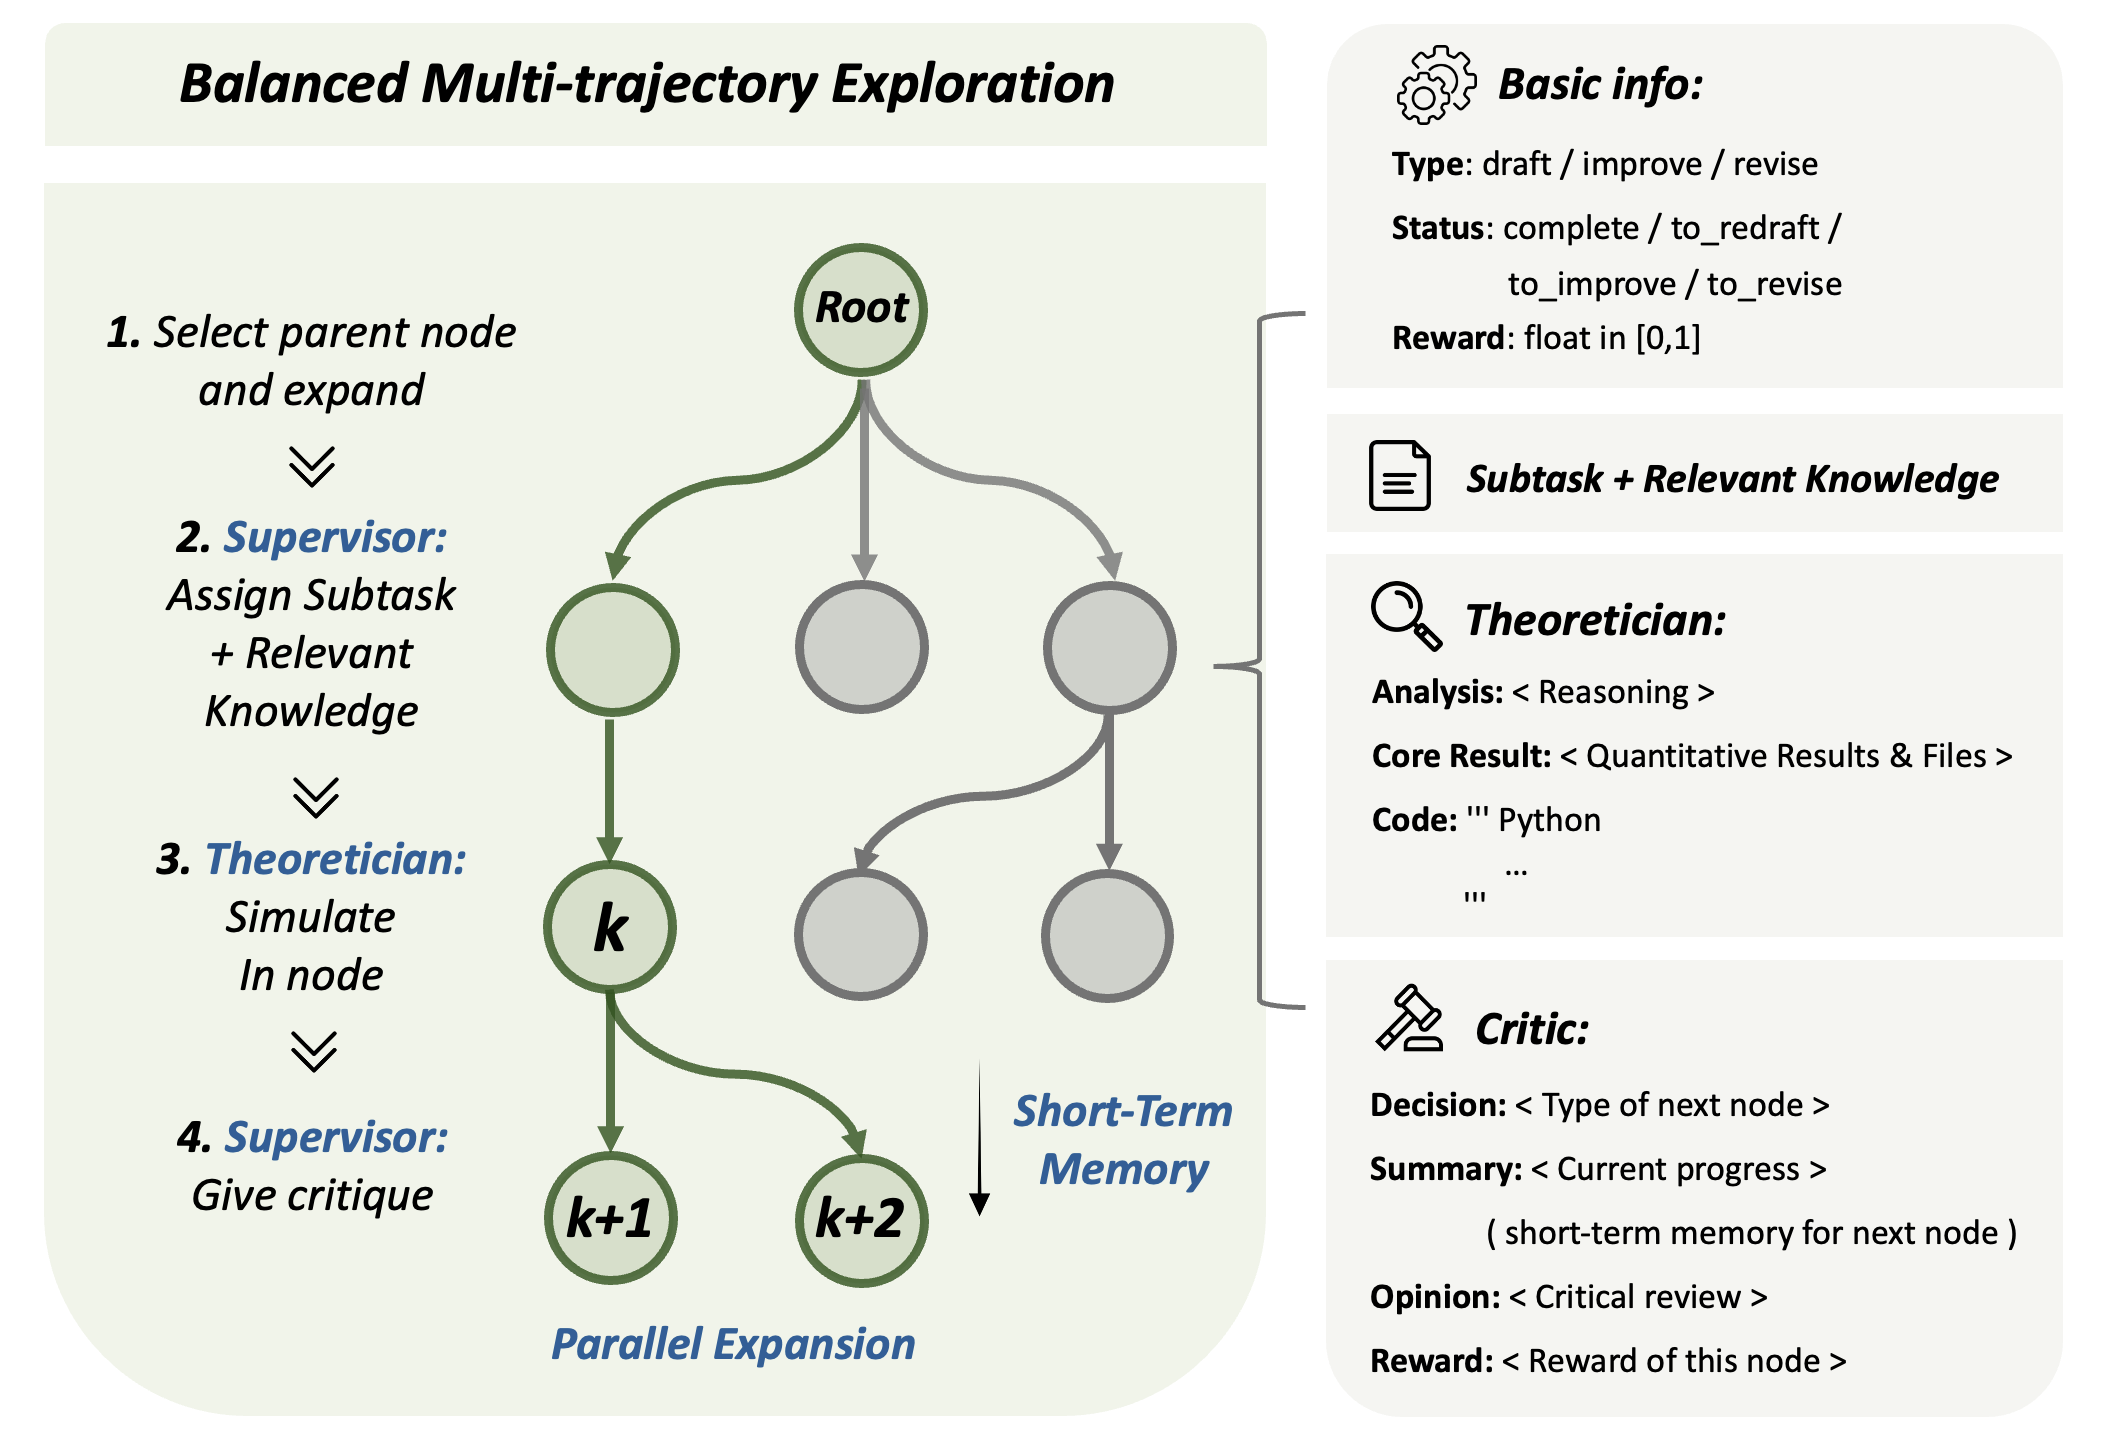
\includegraphics[width=0.78\linewidth]{figure/exploration.jpg}
    \caption{The MCTS Exploration and Node Info}
    \label{fig:mcts}
\end{figure}


\noindent \textbf{a. MCTS-based flexible task scheduling under ultra-long horizons}

As mentioned previously, the raw query is decomposed into executable subtasks by the clarifier before task execution, and these subtasks are individually assigned to MCTS nodes. Along with each subtask, the assigned MCTS node is provided with (a) a concise summary of relevant prior exploration results (primarily inherited from the parent node), and (b) RAG-based background knowledge required for the current subtask, ensuring the completeness and comprehensiveness of the available information. Task decomposition and flexible scheduling enable ultra-long-horizon tasks to be completed through iterative execution, while selectively scoped information, rather than the raw full history, effectively addresses the challenges of context management.

\noindent \textbf{b. Hierarchical collaboration and node-level progress management}

More concretely, two agents collaborate hierarchically during task execution:
\begin{itemize}
    \item \textbf{Supervisor}: Operates independently of individual nodes and is responsible for flexible scheduling and progress management. It performs:
    \begin{itemize}
        \item \textbf{Scheduling / Progress Management}: Decides the subtask to be assigned to MCTS node and provide current progress and provide RAG-based background knowledge needed for the current subtask.
        \item \textbf{Evaluation / Summarizing}: Invokes the knowledge base to rigorously evaluate and summarize the Theoretician's output.
    \end{itemize}
    \item \textbf{Theoretician}: For each assigned subtask, the Theoretician constructs theoretical models, performs analytical reasoning, or translates models into executable code for numerical computation.
\end{itemize}

\noindent \textbf{c. Grounded Feedback as the Foundation for Reliable MCTS Exploration}

A decisive factor for successful long-horizon iteration is obtaining correct feedback signals, since the guidance for refinement and expansion is essential. In the MCTS Exploration of \agent, RAG-Based factual feedback is produced by the supervisor as a critic: it (i) assigns scalar rewards, (ii) determines the types of subsequent nodes, (iii) summarizes the current exploration state to preserve the minimal information needed and (iv) actionable critique to guide next step. The information above are fed back into the tree policy to guide subsequent selection and expansion.

\noindent \textbf{d. MCTS for Broad and Diverse Exploration}

During tree search, nodes are selected using UCT (Upper Confidence bounds applied to Trees) scores, and the structured search tree is expanded iteratively. The UCT value for a node \( v \) is calculated as:
\[
\text{UCT}(v) = \frac{Q_v}{N_v} + C \cdot \sqrt{\frac{\ln N_{\text{parent}}}{N_v}},
\]
where \( Q_v \) is the total reward accumulated for the node, \( N_v \) is the number of visits to the node, \( N_{\text{parent}} \) is the number of visits to its parent, and \( C \) is a constant that controls the trade-off between exploration and exploitation. 

MCTS provides a principled mechanism to (i) exploit high-reward partial solutions, while (ii) continuing to explore under-investigated alternatives to avoid premature convergence. This tree-structured exploration is especially beneficial in long-horizon settings because the search tree itself serves as an externalized record of diverse trajectories. By prioritizing under-explored paths through UCT and supporting parallel multi-trajectory expansion, MCTS enhances efficiency and scalability in navigating vast solution spaces typical of physics problems.

\subsection{\textsc{LANDAU}: Layered Academic Data Universe}

In honor of the eminent universal physicist Lev Landau, we propose \knowledge, the \emph{Layered Academic DAta Universe
} affiliated to \agent, which is designed to navigate \agent and consists of three layers:

\[
LANDAU = \mathcal{L} \cup \mathcal{M} \cup  \mathcal{P},
\]
where $\mathcal{L}$, $\mathcal{M}$, $\mathcal{P}$ denote library, priors, methodology, respectively.

We define these layers as follows:

\begin{itemize}
    \item \textbf{Library $\mathcal{L}$}: Knowledge extracted  from the precise retrieved papers.
    \item \textbf{Methodology $\mathcal{M}$}: Validated effective reasoning path either manually curated or extracted from each successful task, enabling efficient reuse in familiar domains.
    \item \textbf{Priors $\mathcal{P}$}: Manually curated high-confidence knowledge, including concise verified conclusions or distilled textbook/authoritative papers. Such priors are essential in enhancing the reliability of the critic and preventing potential fundamental errors.
\end{itemize}

The library $\mathcal{L}$ is evolving via the accumulation of local library $\mathcal{L}_{Local}$. After each task, the task-specific library $\mathcal{L}_{Local}$ built via literature retrieval are integrated into $\mathcal{L}$; that is
\[
\mathcal{L} \leftarrow \mathcal{L} \cup  \mathcal{L}_{Local}.
\]

Similarly, for the Methodology component $\mathcal{M}$, upon successful task completion, validated effective reasoning trajectories and technical details are summarized, structured, and archived as methodology $\mathcal{M}_{i}$ for future reuse; that is
\[
\mathcal{M}  \leftarrow \mathcal{M}  \cup \{ M_{i} \}.
\]

Such continual accumulation enriches long-term knowledge and enables the autonomous evolution of \knowledge towards comprehensive domain-specific knowledge base.


\section{Case Analysis: Acceleration, Automation and Autonomous Discovery}
\label{sec:case}

In physics---a foundational discipline characterized by high abstraction, intrinsic complexity, and substantial intellectual demand---the research inevitably faces several persistent challenges:

\vspace{-1.6ex}
\begin{itemize}
    \item \textbf{Time dominated by repetitive engineering.} A nontrivial fraction of research hours is spent on labor-intensive yet low-level tasks, such as repeatedly implementing numerical solvers and conducting long cycles of manual hyperparameter tuning.
    \item \textbf{An exceptionally long path from ideas to verifiable conclusions.} Translating a concept into a defensible result typically requires a prolonged pipeline---idea $\rightarrow$ derivation $\rightarrow$ repeated numerical experiments $\rightarrow$ rigorous comparison to prior literature---often spanning months before a final judgment can be made.
    \item \textbf{High abstraction and experience-dependent insight.} Theoretical progress is frequently driven by tacit expertise, intuition, and hard-earned scientific taste, making discovery uneven and difficult to scale.
\end{itemize}
\vspace{-1.6ex}

Correspondingly, we distill three representative problem classes from real-world physics research workflows, ordered by increasing degrees of autonomy:

\vspace{-1.6ex}
\begin{enumerate}
    \item \textbf{Acceleration:} The labor-intensive engineering components of physics research (e.g., coding, debugging, and standard numerical routines) where methods basically well-established and outcomes are relatively predictable. We expect \agent to eliminate the barrier to mastering trivial techniques and liberate the talented researchers from tedious, repetitive engineering tasks.
    \item \textbf{Automation:} Semi-open problems with moderate novelty. Given a human-specified hypothesis, plan, and a selected class of methods, we expect \agent to automatically execute the exploration loop, running experiments, validating hypotheses, and iterating efficiently, thereby substantially compressing the end-to-end research cycle.
    \item \textbf{Autonomous discovery.} Starting from empirical phenomena or scientific challenges, conduct fully independent exploration: propose hypotheses, design and run validation protocols, and iterate towards convincing result, realizing the leap from an AI co-scientist to an AI auto-scientist.
\end{enumerate}
\vspace{-1.6ex}

Starting from empirical phenomena or problems remaining open, conduct fully independent exploration---propose hypotheses, design and conduct validations, and iterates---realizing the transition from an AI co-scientist to an AI auto-scientist.

\subsection{Acceleration: Lattice Extraction of the Collins-Soper Kernel (CS Kernel) from Quasi-TMD Wave Function}

\noindent \textbf{Background and Motivation}

Lattice QCD (LQCD) provides a first-principles, nonperturbative framework for computing
hadronic observables by evaluating the QCD path integral on a discretized Euclidean spacetime
using Monte Carlo techniques~\cite{Wilson:1974sk,Gattringer:2010zz}.
Within this framework, transverse-momentum–dependent observables (TMDs) and their rapidity
evolution are characterized by the Collins--Soper (CS) kernel $K(b_\perp,\mu)$~\cite{Collins:2011zzd},
whose nonperturbative behavior at large $b_\perp$ can be accessed through lattice methods.

The present study addresses the stage of the LQCD workflow that transforms Euclidean correlators
into continuum-like quasi observables and, subsequently, into the CS kernel.
This transformation relies on a controlled sequence of renormalization, large-momentum analysis,
and Fourier transformation steps consistent with the LaMET framework~\cite{Ji:2013dva,Ji:2014gla,Ji:2020ect},
and is used here as a representative application of the automated analysis pipeline.


\noindent \textbf{Methodology: The Automated Lattice Workflow}

In this section we summarize the full lattice-QCD workflow executed by the \agent to extract the Collins--Soper (CS) kernel from quasi-TMD wave functions of the pion.  The system performs an end-to-end chain of operations, starting from raw Euclidean two-point correlators and Wilson-loop data provided by Ref.~\cite{Tan:2025ofx}, and ending with a statistically and systematically controlled lattice determination of $K(b_\perp,\mu)$ at fixed transverse separation.  The individual stages of the computation follow closely the theoretical structure of LaMET factorization and lattice TMD renormalization~\cite{Ji:2019sxk,Ebert:2019okf,Schlemmer:2021aij}.

\noindent \textbf{a. Extraction of Bare Quasi-TMD Matrix Elements}

\begin{figure}[ht]
\centering
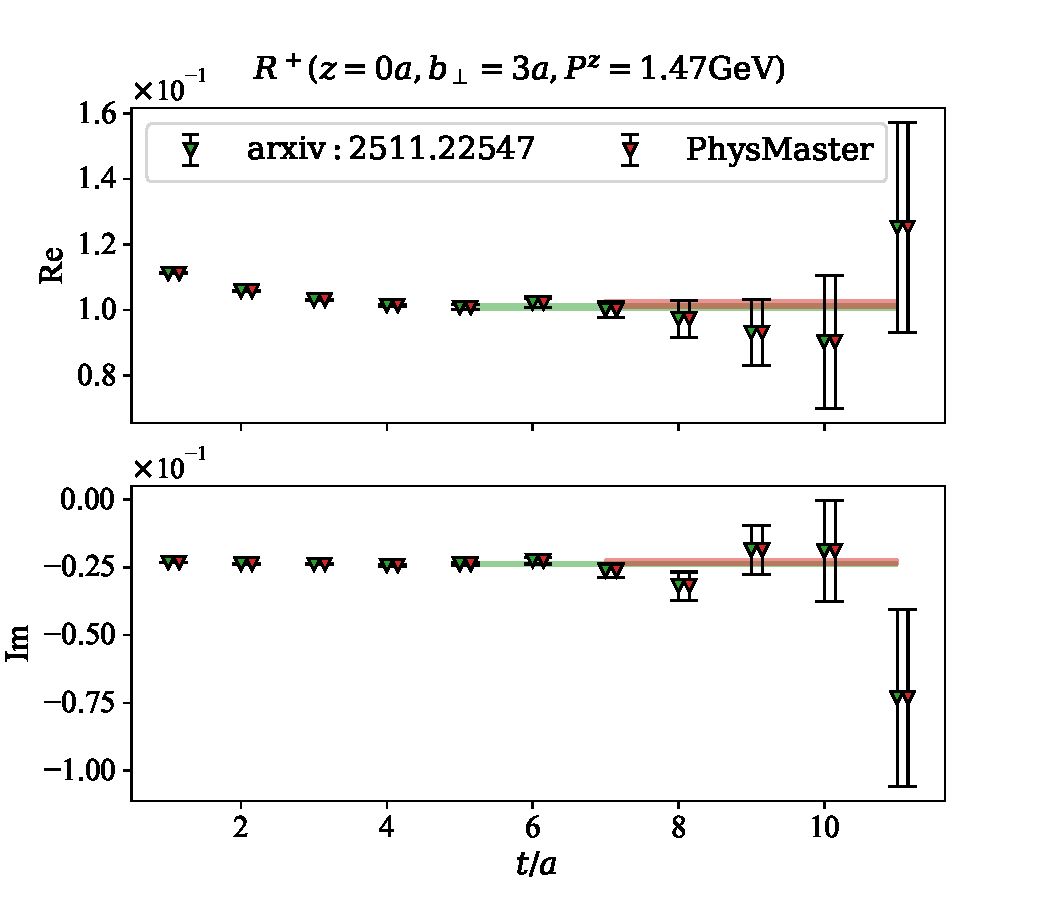
\includegraphics[width=0.45\textwidth]{figure/fit_2pt_ratio_0.pdf}
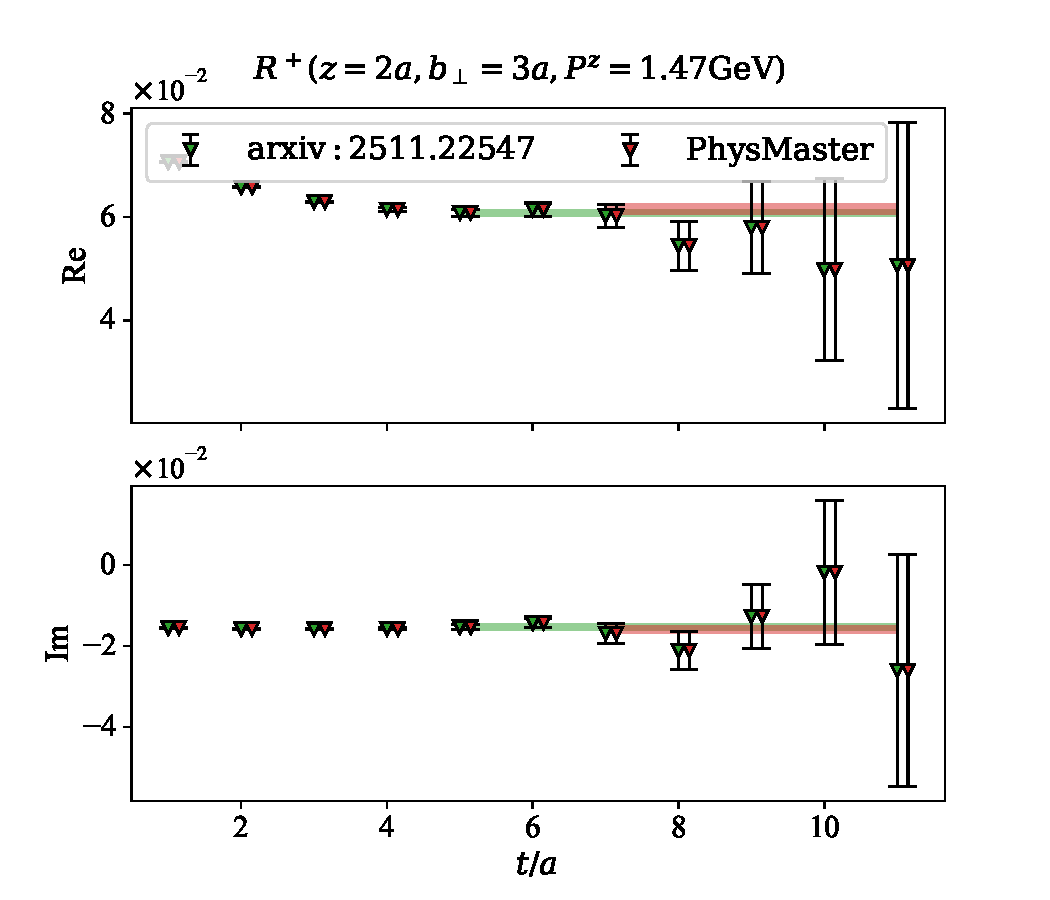
\includegraphics[width=0.45\textwidth]{figure/fit_2pt_ratio_1.pdf}
\caption{Comparison of the nonlocal two-point correlator ratios used to extract the bare
quasi-TMD wave-function matrix elements.
Results obtained using the original analysis of Ref.~\cite{Tan:2025ofx} are compared with those produced by the automated \agent pipeline,
for $P_z=1.47~\mathrm{GeV}$, $z=\{0,2\}a$, and $b=3a$.
The agreement demonstrates the reliability of \agent in reproducing
established lattice fitting results.} 
\label{fig:2pt_fit}
\end{figure}

The starting point is the nonlocal two-point correlator
\(
C_{\text{nl}}(z,b;t)
\),
constructed with a quark bilinear separated by longitudinal distance $z$ and transverse displacement $b_\perp$. Such nonlocal Euclidean correlators with staple-shaped gauge links define quasi-TMD
wave functions in the LaMET framework and have been extensively studied in recent lattice investigations~\cite{Ji:2014gla,Ebert:2019okf,LatticeParton:2020uhz}. For each momentum $P^z=\{4,6\}$ in lattice units, \agent calculate the ratio
\begin{equation}
    R(z,b;t)=\frac{C_{\text{nl}}(z,b;t)}{C_{\text{loc}}(t)}
\end{equation}

removes the dominant time dependence related to the hadron energy.

To isolate the single-hadron matrix element, \agent performs either a one-state or two-state fit:
\begin{equation}
    R(z,b;t)\xrightarrow[t\to\infty]{} \tilde{\Phi}_{\text{bare}}(z,b) ,
\end{equation}
where the fit range is selected automatically using log-effective-plateau diagnostics combined with covariance-aware $\chi^2/\mathrm{dof}$ ranking.  

\begin{figure*}[ht]
\centering
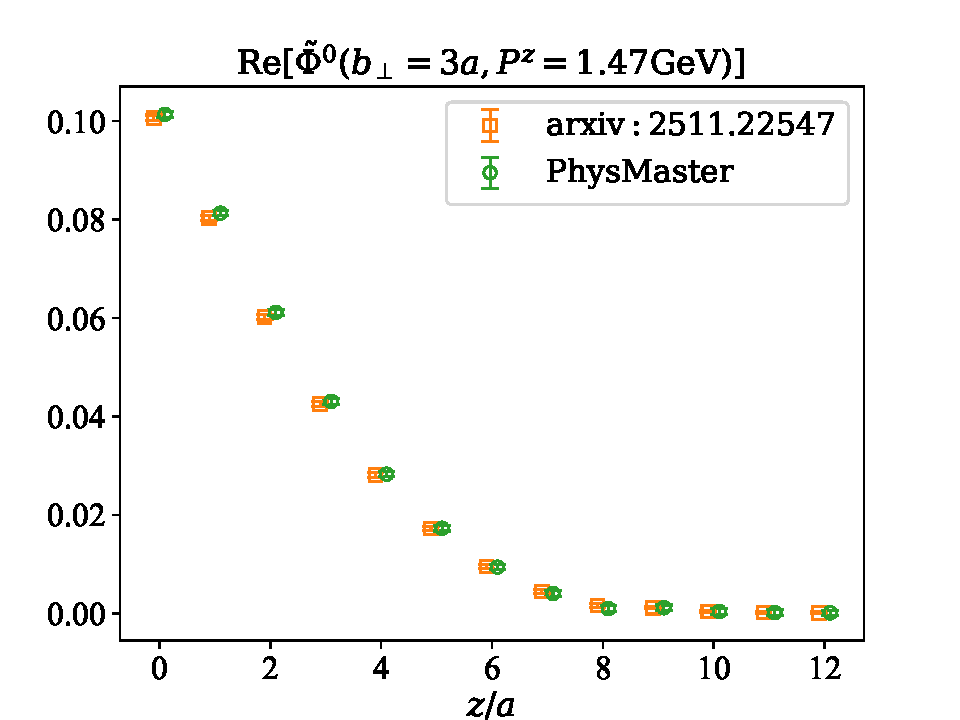
\includegraphics[width=0.45\textwidth]{figure/bare_Pz4_b3_re.pdf}
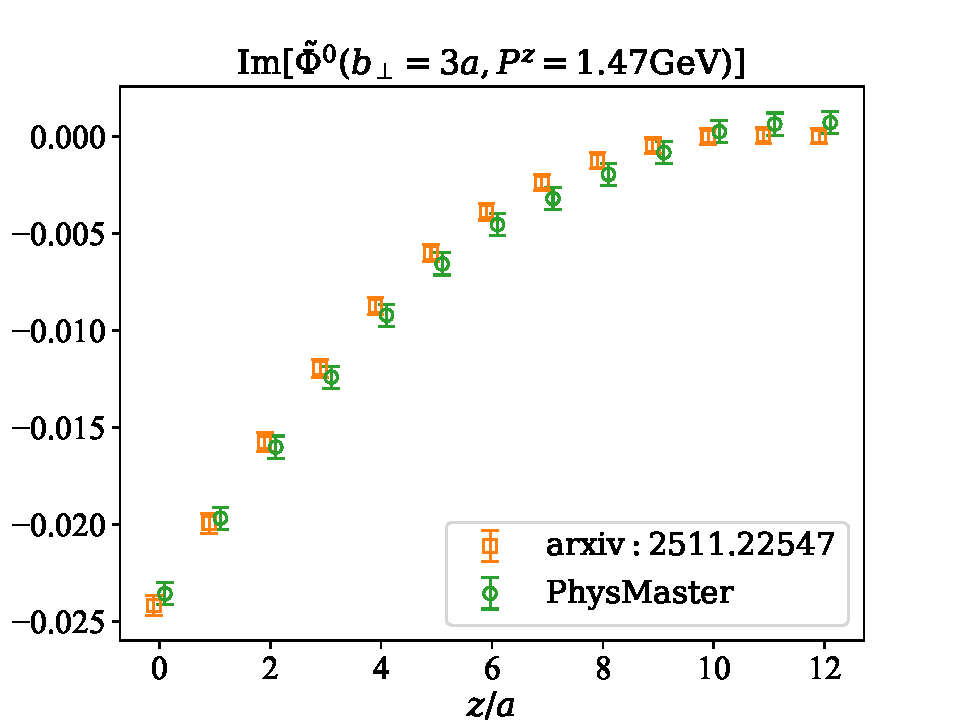
\includegraphics[width=0.45\textwidth]{figure/bare_Pz4_b3_im.pdf}
\caption{Coordinate-space distributions of the bare quasi-TMD wave-function matrix elements
at $P_z=1.47~\mathrm{GeV}$ and transverse separation $b=3a$.
Left and right panels show the real and imaginary parts, respectively.
Results from Ref.~\cite{Tan:2025ofx} and \agent are consistent within statistical
uncertainties over the full range of longitudinal separations.} 
\label{fig:coord_space_distribution}
\end{figure*}

\begin{figure*}[ht]
\centering
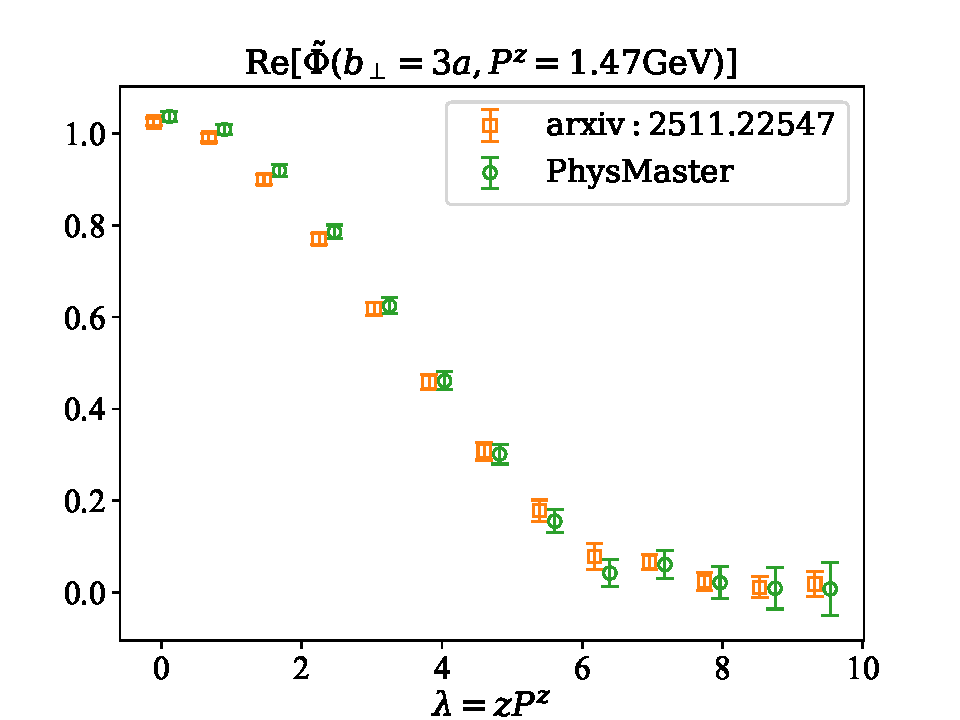
\includegraphics[width=0.45\textwidth]{figure/Pz4_b3_re.pdf}
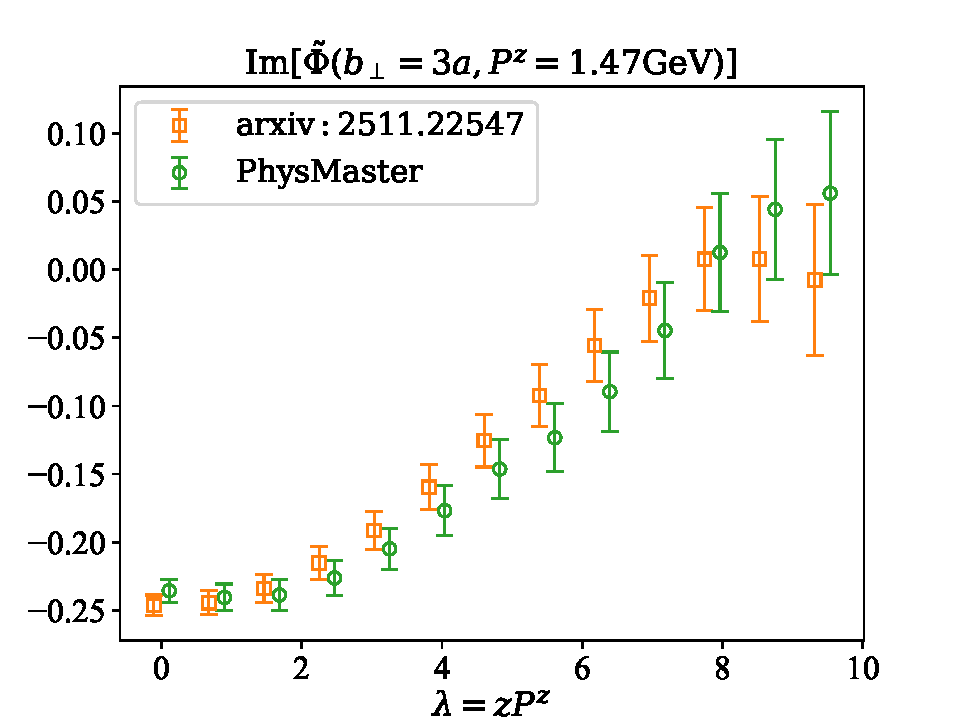
\includegraphics[width=0.45\textwidth]{figure/Pz4_b3_im.pdf}
\caption{Renormalized coordinate-space quasi-TMD wave-function matrix elements at
$P_z=1.47~\mathrm{GeV}$ and $b=3a$, obtained after dividing by the Wilson-loop
renormalization factor $Z_E$.
The removal of the linear divergence leads to a significantly improved large-$z$
behavior compared to the bare results.} 
\label{fig:ren_coor}
\end{figure*}

Fig.~\ref{fig:2pt_fit} presents a comparison between the results obtained using Ref.~\cite{Tan:2025ofx} and those from \agent for extracting the matrix element at $ P_{z}=1.47\mathrm{GeV}$, $z=\{0,2\}a$, and $b=3a$. The raw data and the corresponding fitted results from both approaches agree within uncertainties, indicating that \agent can reliably handle large-scale and otherwise tedious fitting tasks, while automatically determining a reasonable fit window.

This yields the full coordinate-space distribution of the bare quasi-TMDWF matrix element for all integer $z\in[-12,12]a$.
Fig.~\ref{fig:coord_space_distribution} displays the coordinate-space profile of the bare matrix elements at $P_{z}=1.47~\text{GeV}$ and $b=3a$, as obtained from both Ref.~\cite{Tan:2025ofx} and \agent. The real and imaginary components extracted from the two methods exhibit mutually compatible behavior within statistical uncertainties.

\noindent \textbf{b. Renormalization Using the Wilson Loop $Z_E$}

To remove the linear divergence of the staple-shaped gauge link, the computation uses the nonperturbative renormalization prescription~\cite{Dotsenko:1979wb,Ji:2017oey,Ebert:2018gzl}
\begin{equation}
    \tilde{\Phi}_{\mathrm{ren}}(z,b)
=
\frac{\tilde{\Phi}_{\mathrm{bare}}(z,b)}
     {\sqrt{Z_E(z+2L,b)}},
\qquad L=6a,
\end{equation}
where $Z_E$ is supplied as the expectation value of Wilson loops with longitudinal length $z+2L$ at fixed transverse separation $b=3a$. Thus, the results shown in Fig.~\ref{fig:ren_coor} indicate that \agent identifies the correct $z+2L$ entry for each matrix element and performs the renormalization pointwise.   

\noindent \textbf{c. Asymptotic Continuation at Large $\lambda = z P^z$}

At large $\lambda$ the lattice signal suffers exponential noise degradation.  
\agent stabilizes the correlator tail through a physics-motivated joint fit to the expected LaMET asymptotic form~\cite{Ji:2013dva,Izubuchi:2018srq,Alexandrou:2020zbe}:
\begin{equation}
    \tilde{\Phi}(\lambda,b_\perp)
=
\left[
\frac{c_1}{(-i\lambda)^{n_1}}
+
e^{i\lambda}
\frac{c_2}{(i\lambda)^{n_2}}
\right]
e^{-\lambda/\lambda_0}.
\end{equation}

A simultaneous fit to the real and imaginary parts is carried out over a sliding window of large $\lambda$, with Bayesian priors enforcing smoothness and positivity constraints on $\lambda_0$.  

\begin{figure}[ht]
\centering
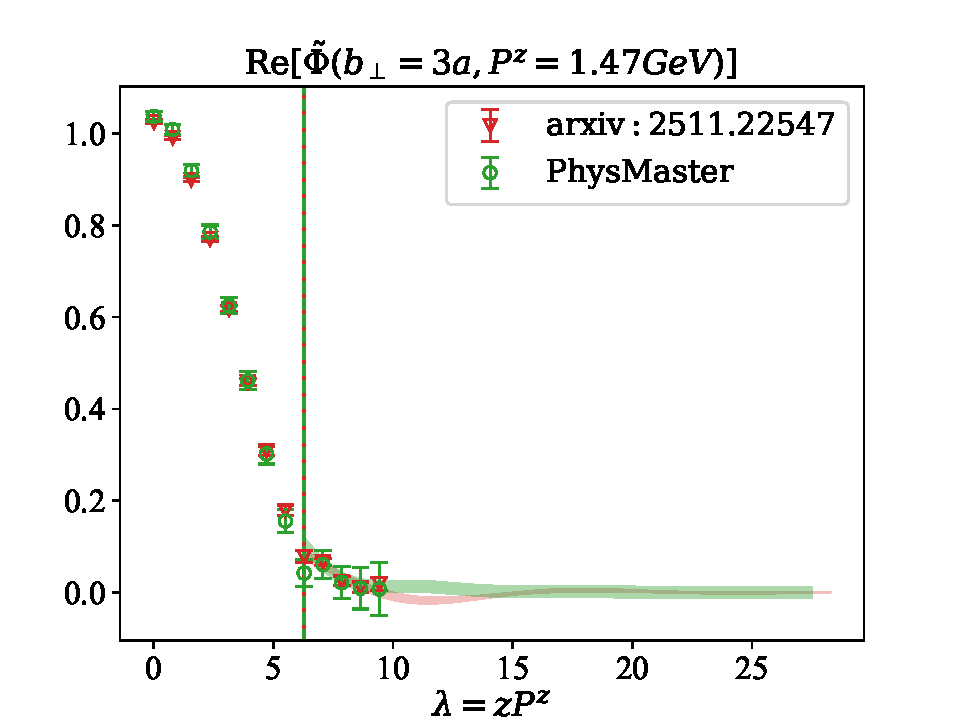
\includegraphics[width=0.45\textwidth]{figure/extrap_Pz4_b3_re.pdf}
\caption{Large-$\lambda$ continuation of the renormalized quasi-TMD matrix elements at
$P_z=1.47~\mathrm{GeV}$ and $b=3a$.
Solid curves denote the physics-motivated asymptotic fits used to replace noisy
lattice data at large separations.
Results from Ref.~\cite{Tan:2025ofx} and \agent illustrate different continuation
strategies while exhibiting consistent asymptotic suppression.} 
\label{fig:extrap}
\end{figure}

The fitted asymptotic tail replaces the noisy data beyond the breakdown point, producing a smoothly continued coordinate-space matrix element $\tilde{\Phi}(\lambda,b)$ valid over an extended domain. Fig.~\ref{fig:extrap} presents the extrapolated coordinate–space matrix elements at $b = 3a$ and $P_{z} = 1.47~\text{GeV}$ obtained from both Ref.~\cite{Tan:2025ofx} and \agent. As is evident from the comparison, the extrapolation performed in Ref.~\cite{Tan:2025ofx} is noticeably more conservative. In contrast, \agent is capable of enforcing a prescribed asymptotic behavior while performing the continuation. Although the two approaches differ in the oscillatory region, both extrapolated curves consistently approach zero at large separations.


\noindent \textbf{d. Fourier Transform to Momentum Space}

The quasi-TMD wave function in momentum space is defined as~\cite{Radyushkin:2017cyf,Lin:2017snn}
\begin{equation}
    \tilde{f}(x,b_\perp,P^z)
=
\int \frac{d\lambda}{2\pi}\,
e^{i(x-\tfrac12)\lambda}\,
\tilde{\Phi}(\lambda,b_\perp).
\end{equation}

After replacing the unstable large-$\lambda$ signals with the extrapolated values and discretizing the above formula, \agent produced the results shown in the left panel of Fig.~\ref{fig:WF_mom}. The comparison indicates that the real parts obtained from Ref.~\cite{Tan:2025ofx} and \agent exhibit noticeable differences within the physical region $x \in [0,1]$, while the imaginary parts remain largely consistent. This discrepancy in the real part can be attributed to the different extrapolation schemes applied at large $\lambda$, and it is typically accounted for as a source of systematic uncertainty.

\begin{figure}[ht]
\centering
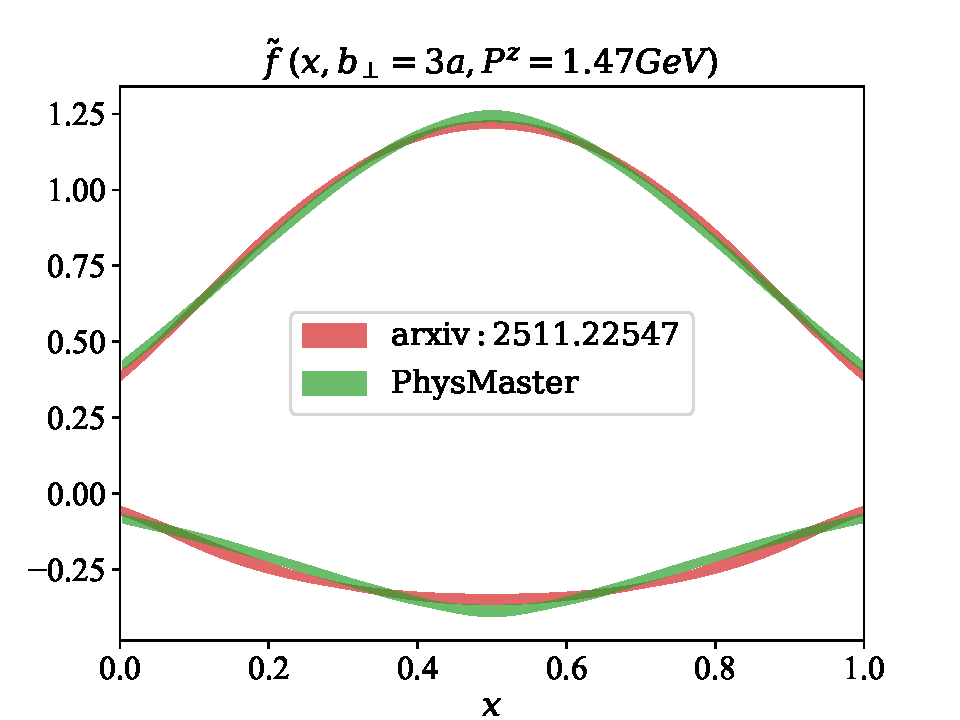
\includegraphics[width=0.45\textwidth]{figure/WF_Pz4_b3.pdf}
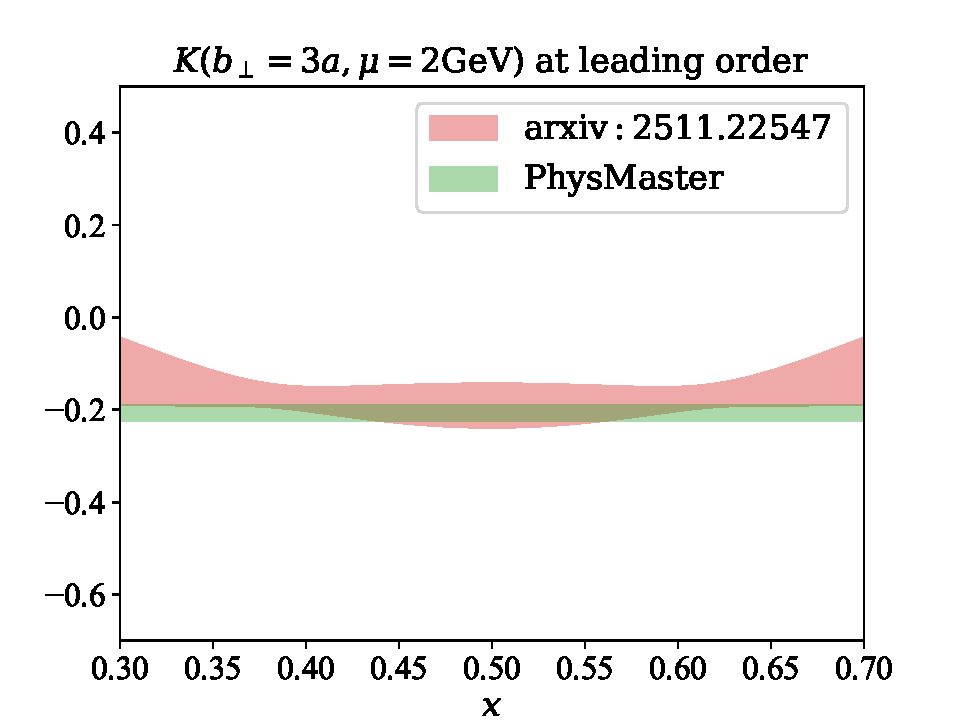
\includegraphics[width=0.45\textwidth]{figure/K.pdf}
\caption{Left panel: Momentum-space quasi-TMD wave functions $\tilde{f}(x,b_\perp,P^z)$ at
$P_z=1.47~\mathrm{GeV}$ and $b=3a$ obtained after Fourier transformation, where the up two are the real part and the down are imaginary part. Right panel: CS kernel $K(b_\perp,\mu)$ extracted from quasi-TMD wave functions. Results from Ref.~\cite{Tan:2025ofx} and \agent are consistent in their central values, while the automated pipeline yields reduced statistical uncertainties.} 
\label{fig:WF_mom}
\end{figure}

\noindent \textbf{e. Extraction of the Collins--Soper Kernel}

Finally, \agent evaluates the tree-level LaMET ratio~\cite{Ji:2014gla,Ebert:2018gzl,Ji:2019sxk}
\begin{equation}
    K(b_\perp,\mu)
=
\frac{1}{\ln(P_1^z/P_2^z)}
\ln\!\left[
\frac{\tilde{f}(x,b_\perp,P_1^z)}
     {\tilde{f}(x,b_\perp,P_2^z)}
\right],
\end{equation}
which holds because the hard coefficients obey $H^\pm(\zeta_1,\mu)=H^\pm(\zeta_2,\mu)=1$ at tree level~\cite{Ebert:2019okf,Ji:2019sxk,LatticePartonLPC:2023pdv,LatticeParton:2020uhz}.

For each $x\in(0,1)$ the kernel is computed with full covariance propagation.  
\agent then removes the residual $x$ dependence by:
\begin{itemize}
    \item fitting $K(x)$ to a constant plateau in the central $x$ region,
    \item performing a correlated average weighted by the inverse covariance.
\end{itemize}

The right panel of Fig.~\ref{fig:WF_mom} presents a comparison between the Collins--Soper kernel extracted using Ref.~\cite{Tan:2025ofx} and \agent. The two central values of $K(b_\perp{=}3a,\mu)$ are consistent within uncertainties. However, the statistical errors from \agent are noticeably smaller, which may be due to the neglect of systematic uncertainties arising from the extrapolation procedure.




\noindent \textbf{Discussion}

The results above illustrate that \agent provides an efficient and robust framework
for automating complex lattice-QCD analyses.
Starting from raw two-point correlators and Wilson-loop inputs,
the pipeline executes all essential stages—from correlator fitting and renormalization
to large-$\lambda$ stabilization, Fourier transformation, and LaMET matching—in a
consistent and reproducible manner, substantially reducing manual intervention.

A key strength of \agent lies in its scalability.
As the dimensionality of the problem increases, for example through additional
momenta, lattice ensembles, or operator structures, the framework can process
the resulting datasets efficiently while maintaining statistical stability and
reproducibility.
Automated selections of fit ranges and continuation parameters further limit
human bias, leading to reduced statistical fluctuations relative to traditional
manual workflows.

The CS-kernel analysis presented here constitutes only a limited demonstration
of the capabilities of \agent.
The primary objective is not the CS kernel itself, but the acceleration and
standardization of the entire lattice QCD analysis workflow.
Future developments will focus on automated treatments of systematic uncertainties
and extensions to broader classes of observables, multiple lattice spacings,
and continuum extrapolations.
In this sense, the present study serves as a proof of principle, and readers are
invited to anticipate more comprehensive applications of \agent to large-scale
lattice QCD computations.





\subsection{Acceleration: Ab Initio Calculation of The First Excitation Energy of Lithium Atoms}

%% Background
\noindent \textbf{Background and Motivation}

The variational method is a cornerstone of quantum mechanics, providing a rigorous upper bound to the ground-state energy of many-body systems, as described in standard texts by Ref. \cite{Griffiths:2018} and Ref.\cite{Levine:2013qj}. 
While modern quantum chemistry relies heavily on established software packages (e.g., the Gaussian suite of \cite{Gaussian16} and the PySCF framework by \cite{Sun:2018}) using Gaussian-type orbitals (GTOs) as pioneered by \cite{Boys:1950}, 
constructing a solver \textit{ab initio}—starting from the analytical evaluation of integrals and basis set design—remains a fundamental exercise in theoretical physics. Crucially, this evaluation precludes access to external global knowledge bases or literature searches, thereby isolating the agent's intrinsic ability to reason through the Hamiltonian's structure, justify approximations, and ensure numerical robustness purely from first principles.
% It tests the rigorous understanding of the underlying Hamiltonian, the validity of approximations, and numerical stability.

The specific scientific problem addressed here is the calculation of the first electronic excitation energy of the neutral Lithium atom (Li, $Z=3$), corresponding to the transition $1s^2 2s^1 \to 1s^2 2p^1$.
This requires solving the Schrödinger equation for a three-electron system under the Born-Oppenheimer approximation.
Unlike routine computations, this task imposes a strict constraint: the solver must be built from scratch using only the Julia standard library, 
forcing the autonomous agent to derive, implement, and optimize the necessary theoretical components—including basis set construction, angular momentum algebra, and numerical integration schemes—without black-box dependencies.

%% Obstacles
\noindent \textbf{Obstacles}

Solving this problem autonomously involves overcoming significant theoretical and algorithmic barriers:

\vspace{-1.6ex}
\begin{itemize}
    \item \textbf{Theoretical Derivation:} The agent must correctly derive the energy functionals for open-shell doublet states. This involves handling two-electron Coulomb ($J$) and Exchange ($K$) integrals, where specific angular momentum coupling coefficients (e.g., the factor of $1/3$ in the $s$-$p$ exchange interaction) must be rigorously determined using the coupling schemes of Ref. \cite{condon1935theory}.
    \item \textbf{Numerical Singularity and Tails:} The radial integrals involve evaluating wave functions from the nucleus ($r \to 0$, where $1/r$ potentials diverge) to the asymptotic tail ($r \to \infty$). Naive integration schemes often fail to capture both regimes efficiently.
    \item \textbf{Basis Set Design:} Without access to pre-tabulated basis sets  (like the STO-3G set defined by Ref.\cite{Hehre:1969}), the agent must construct a minimal, physically motivated basis (Slater-Type Orbitals) and implement an optimization strategy to find the variational parameters that minimize the energy.
\end{itemize}
\vspace{-1.6ex}

Manually deriving these formulas and writing a bug-free, optimized numerical integrator typically requires days of effort for a graduate student.

%% Methodology
\noindent \textbf{Methodology}

The workflow proceeded in three distinct, self-correcting stages: Theoretical Construction, Algorithmic Implementation, and Critical Verification.

\medskip
{a. Theoretical Construction and Basis Design.}
First, the physical model was established by selecting Slater-Type Orbitals (STOs), $R_{n,l}(r) \propto r^{n-1}e^{-\zeta r}$, as the basis functions. These were chosen for their correct cusp behavior at the nucleus, which offers superior convergence compared to GTOs for minimal basis
calculations, as analyzed by Ref.\cite{Slater:1930}.
Energy expressions for the doublet configurations were derived as follows:
\begin{align*}
    E(1s^2 2s) &= 2h_{1s} + h_{2s} + J_{11} + 2J_{12} - K_{12} \\
    E(1s^2 2p) &= 2h_{1s} + h_{2p} + J_{11} + 2J_{1p} - K_{sp}
\end{align*}
Crucially, for the $s$-$p$ exchange integral $K_{sp}$, the contribution was identified as arising solely from the $k=1$ term in the multipole expansion, with the prefactor $1/3$ derived from the integration over spherical harmonics.

\medskip
{b. Numerical Implementation.}
To handle the semi-infinite integration domain $[0, \infty)$, a non-uniform grid mapping was implemented:
\[
    r(s) = \frac{s}{1-s}, \quad s \in [0, 1).
\]
This transformation maps the infinite range to a finite interval while naturally concentrating grid points near the nucleus ($s \to 0$), thereby improving the accuracy for the nuclear potential $V \propto -Z/r$.

For the two-electron integrals, which formally scale as $O(N^2)$, an efficient $O(N)$ algorithm was implemented utilizing the split-domain identity for the radial multipole expansion found in Ref.\cite{Szabo:1996}:
\[
    I_k[f,g] = \int_0^\infty dr_1 f(r_1) \left[ r_1^{-1-k} \mathcal{B}(r_1) + r_1^k (\mathcal{C}(\infty) - \mathcal{C}(r_1)) \right],
\]
where $\mathcal{B}$ and $\mathcal{C}$ are cumulative integrals of the density $g(r)$. 
Additionally, a Gram-Schmidt orthogonalization routine was implemented to ensure that the $1s$ and $2s$ orbitals remained orthogonal ($\langle 1s | 2s \rangle = 0$) despite being defined by distinct variational exponents $\zeta$.

\medskip
{c. Optimization and Verification.}
A nested grid-search algorithm was employed to optimize the exponents. 
The ground state parameters $(\zeta_1, \zeta_2)$ were optimized first, followed by the optimization of the excited state parameter $\zeta_p$ with $\zeta_1$ fixed at its ground-state value.
Following the implementation, the theoretical framework and workflow underwent a rigorous verification process. Analytical normalization constants were verified, the absence of the $k=2$ term in the direct $s$-$p$ interaction was confirmed to be theoretically consistent, and the stability of the integration grid ($N=4001$ points) was validated.

%% Conclusion
\noindent \textbf{Conclusion}

The agent successfully constructed a full-stack variational solver and computed the following energies:
\begin{itemize}
    \item Ground State ($1s^2 2s$): $E_g = -7.4178$ Ha (Optimized $\zeta_{1s}=2.68$, $\zeta_{2s}=0.63$).
    \item Excited State ($1s^2 2p$): $E_e = -7.3504$ Ha (Optimized $\zeta_{2p}=0.52$).
\end{itemize}
The resulting first excitation energy is:
\[
    \Delta E = 0.0675 \text{ Hartree}.
\]
This result is in remarkable agreement with the experimental value of approximately $0.0679$ Ha ($\sim 1.85$ eV) from the database of Ref.\cite{NIST_ASD}, with a deviation of only $0.0004$ Ha. 
This high accuracy, achieved with a minimal basis set, demonstrates the agent's ability to not only write code but to perform high-level physical reasoning—correctly handling angular momentum algebra, designing stable numerical schemes, and rigorously optimizing variational parameters. 
The work highlights the potential of AI agents to accelerate the "engineering" aspects of theoretical physics, transforming abstract problem statements into high-precision numerical results in a fully autonomous loop, consistent with the general theoretical framework detailed by \cite{sachdev2011quantum}.

While this problem itself is not particularly challenging academically, its significance lies in demonstrating the feasibility of long-horizon, high-rigor, and fully verifiable production-grade scientific computing workflows—an essential prerequisite for closing the loop from physical reasoning, algorithmic implementation, to autonomous research at scale.


\subsection{Automation: Quantum Phase Transition in the Union Jack Bose-Hubbard Model via Quantum Monte Carlo (QMC)}

\noindent \textbf{Background and Motivation}

\agent addresses one of the most challenging problems in quantum many-body physics: the precise determination of the quantum phase transition point in the Union Jack Bose-Hubbard Model (BHM). The BHM serves as the canonical theoretical framework for describing the quantum dynamics of interacting bosons on optical lattices, capturing the competition between kinetic delocalization and interaction-induced localization that drives the zero-temperature Superfluid (SF) to Mott Insulator (MI) quantum phase transition~\cite{fisher1989boson,greiner2002quantum}. The establishment of this framework laid the theoretical groundwork for the research leading to the 2001 Nobel Prize in Physics on Bose-Einstein condensation. While the square lattice has been exhaustively characterized, the isotropic Union Jack lattice, which was constructed by augmenting a square lattice with diagonal next-nearest-neighbor (NNN) hopping, presents a topologically distinct, non-bipartite geometry with a high coordination number of $z=8$.

Determining the critical ratio $(t/U)_c$ on such highly connected architectures is fundamental for validating universality classes in complex geometries~\cite{lkacki2016locating}. The Hamiltonian governing the system is given by:
\begin{equation}
\op{H} = -t \sum_{\langle i,j \rangle_{\text{NN}}} (\dagop{b}_i \op{b}_j + \text{h.c.}) - t \sum_{\langle\langle i,j \rangle\rangle_{\text{diag}}} (\dagop{b}_i \op{b}_j + \text{h.c.}) + \frac{U}{2} \sum_i \op{n}_i (\op{n}_i - 1) - \mu \sum_i \op{n}_i,
\end{equation}
where the hopping amplitude $t$ is uniform for both nearest-neighbor (NN) and diagonal bonds. The enhanced connectivity ($z=8$) drastically lowers the energy cost for particle delocalization compared to the square lattice ($z=4$), theoretically suppressing the critical point well below the standard square lattice value of $(t/U)_c^{\text{sq}} \approx 0.0597$. Precise numerical benchmarks are required to quantify this suppression and confirm the robustness of the $(2+1)$D XY universality class in the presence of frustration-free triangular loops, consistent with the general theoretical framework detailed by Ref.\cite{sachdev2011quantum}.

\noindent \textbf{Obstacle}

This work is not merely code implementation or parameter scanning; it constitutes a full-stack, algorithmically-driven, Ph.D. thesis-level research effort. The primary obstacle lies in overcoming the severe algorithmic opacity inherent in high-precision Quantum Monte Carlo (QMC), utilizing techniques such as those reviewed by Ref.\cite{sandvik2010computational}. The primary obstacle lies not in the derivation of equations, but in the stochastic engineering required to implement a valid Stochastic Series Expansion (SSE) with directed-loop updates, building upon the original worm algorithm of Ref.\cite{prokofev1998exact} and the directed-loop formulation of Ref.\cite{syljuasen2002quantum}.  \agent was required to autonomously resolve topological subtleties specific to the Union Jack lattice, particularly the non-trivial accounting of winding number topology and the challenge of critical slowing down.

\agent had to autonomously implement a highly optimized Robbins-Monro stochastic root-finding scheme, root-finding scheme, following the method of Ref. \cite{robbins1951stochastic}, to tune the chemical potential $\mu$ against a vanishing compressibility ($\kappa \to 0$) near the critical point---a task where naive bisection fails. Furthermore, extracting the thermodynamic limit requires physical intuition to distinguish genuine finite-size scaling behavior from corrections to scaling. Remarkably, the agent completes this entire research task without any access to global knowledge bases or literature search. This proves its ability to derive every algorithmic detail—from the SSE update weights to the topological constraints—directly from the first principles of the Hamiltonian, demonstrating a capacity for independent scientific discovery and rigorous theoretical reasoning.

The learning curve to master QMC for a Ph.D. student is steep, while a researcher typically needs more than one year to reach a senior level of expertise to effectively apply it. Futhermore, the independent completion of this project, which involves the construction, debugging, and optimization of high-precision QMC code, would conventionally necessitate one to three months' full-time effort. However, the deployment of \agent profoundly accelerates this research cycle, drastically reducing the time commitment required.

\noindent \textbf{Methodology}

\agent employ the Stochastic Series Expansion (SSE) QMC algorithm with directed-loop updates to sample the partition function $Z = \text{Tr}[e^{-\beta \op{H}}]$ without discretization error~\cite{xu2019revealing,wenzel2009comprehensive}. Simulations are conducted on $L \times L$ tori with periodic boundary conditions for system sizes $L \in \{8, 12, 16, 20\}$.

To strictly target the tip of the $n=1$ Mott lobe, \agent operated in the grand-canonical ensemble. The chemical potential $\mu$ was dynamically tuned using a compressibility-driven Robbins-Monro recursion algorithm. At the $k$-th update step, $\mu$ was adjusted as:
\begin{equation}
\mu_{k+1} = \mu_k - \alpha_k \frac{\ave{n}_k - 1}{\kappa_k}, \quad \text{with} \quad \kappa_k = \frac{\beta}{L^2} \text{Var}(N)_k,
\end{equation}
where $\alpha_k$ is a decaying step size sequence. This adaptive method utilizes the on-the-fly measurement of compressibility $\kappa_k$ to stabilize convergence, achieving a density tolerance of $|\ave{n} - 1| \leq 5 \times 10^{-4}$ across all parameter sets.

To probe the quantum critical point (dynamic exponent $z=1$), \textbf{PhysMaster} fixed the aspect ratio $\beta = 1.5 L$ (in units of $1/U$). The critical point was identified via the scaling of the superfluid stiffness $\rho_s \propto \ave{W^2}/\beta$, where $\ave{W^2}$ is the squared winding number. \textbf{PhysMaster} utilized \textbf{single-histogram reweighting} of the kinetic operator count $K$ to interpolate $\ave{W^2}(t)$ continuously, allowing for a precise determination of the crossing location significantly below the simulation grid spacing. Crossing points $t^*(L_1, L_2)$ of the scale-invariant observable $\ave{W^2}$ are determined for successive system sizes. \agent employ single-histogram reweighting of the kinetic operator count $K$ to interpolate $\ave{W^2}(t)$ continuously between simulated grid points ($t \in [0.027, 0.033]$), allowing for a precise determination of the crossing location significantly below the simulation grid spacing.

The thermodynamic limit was extracted by \textbf{PhysMaster} by autonomously extrapolating the finite-size crossing points $t^*(L_1, L_2)$ against the scaling variable $1/\sqrt{L_1 L_2}$:
\begin{equation}
t^*(L_{\text{mid}}) = (t/U)_c + a \cdot (L_{\text{mid}})^{-1/\nu},
\end{equation}
where $L_{\text{mid}} = \sqrt{L_1 L_2}$.

\noindent \textbf{Conclusion}

\agent's achievement is its ability to autonomously execute the entire scientific discovery loop. From physical modeling and high-precision algorithm optimization to complex finite-size scaling extrapolation, it can accomplish the whole task without any human intervention. such an autonomous work establishes the most rigorous numerical benchmark for the Bose-Hubbard model on the isotropic Union Jack lattice. Through the automated integration of SSE directed-loop updates, stochastic $\mu$-tuning, and histogram reweighting, \agent determine the critical point to be:
\begin{equation}
\left(\frac{t}{U}\right)_{c} = 0.02992 \pm 0.00020.
\end{equation}
The small statistical uncertainty ($\sim 0.7\%$) confirms the efficacy of the methodology. Physically, this value represents a $\approx 50\%$ reduction compared to the square lattice critical point ($0.0597$), quantitatively demonstrating the strong stabilization of the superfluid phase driven by the high coordination number ($z=8$). The results are fully consistent with $(2+1)$D XY universality class predictions.



\begin{figure}[ht]
\centering
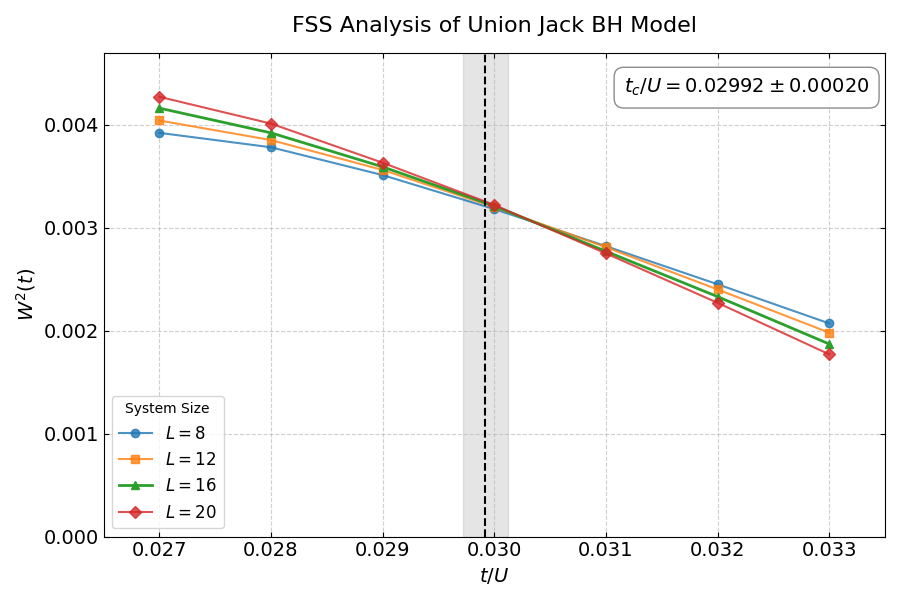
\includegraphics[width=0.6\textwidth]{figure/critical_point.png}
\caption{Finite Size Scaling (FSS) analysis for determining the quantum critical point of the Union Jack BH Model from \agent. The figure shows the scaling of the quantity $W^2(t)$ as a function of the normalized time $t/U$, plotted for various system sizes, $L \in \{8, 12, 16, 20\}$. According to the FSS hypothesis, the curves for different $L$ intersect precisely at the quantum critical point $t_c$. The estimated critical value is $t_c/U = 0.02992 \pm 0.00020$, which is marked by the dashed line and the shaded grey region, demonstrating the uncertainty of the intersection point.} 
\label{fig:cp}
\end{figure}

Most significantly, this result was achieved through an entirely autonomous AI workflow. The agent successfully navigated the full scientific loop: from implementing the correct winding number topology for diagonal bonds to executing high-precision finite-size scaling analysis. This demonstrates an emerging capability for AI systems to independently drive discovery in computational many-body physics, moving from simple code generation to complex, physically motivated algorithmic reasoning. This project serves as a powerful demonstration of how integrated AI systems can dramatically enhance the efficiency and accessibility of computational physics research, setting a new standard for automated scientific discovery.

\newpage
\subsection{Automation: Differential Precession Effects on Nozzle-Shock Dissipation in Tidal Disruption Events (TDEs)}

\noindent \textbf{Background and Motivation}

Tidal Disruption Events (TDEs) occur when a star passes near a supermassive black hole (SMBH; $\sim 10^6 M_\odot$), leading to its complete tidal destruction and formation of an elongated debris stream, roughly half of which falls back toward the black hole. During fallback, the stream accelerates and thins, and near pericenter, fluid elements collide at high relative speeds, dissipating energy in a process known as the nozzle shock. General relativistic effects, including apsidal and nodal precession, further modify stream trajectories and dissipation near rapidly spinning SMBHs. TDEs are central to the frontier of black hole physics, building upon the foundational work recognized by the 2020 Nobel Prize in Physics for confirming the existence of supermassive black holes and validating General Relativity.

Previous studies have largely considered single-energy fallback, ignoring the star's finite size. In reality, different stellar regions experience varying tidal potentials, producing a spread of debris energies and slightly differing geodesics. These multi-energy streams intersect at non-zero angles at the nozzle, combining transverse compression with longitudinal velocity projections, potentially enhancing dissipation. \agent refer to this mechanism, arising from the tidal energy spread, as differential precession.

Since the establishment of the standard TDE framework in the 1980s \citep{carter1983tidal}, theoretical and simulation studies have evolved rapidly, refining the initial models. Traditional theory posits that nozzle shocks near pericenter dissipate significant kinetic energy, aiding accretion disk formation ~\citep{evans1989tidal,shiokawa2015general}. Yet, fully simulating a TDE---from stellar approach and disruption to stream formation, collisions, disk circularization, and radiation---requires comprehensive GR magnetohydrodynamics (MHD) with radiative transfer, exceeding current computational capabilities ~\citep{dai2018unified,curd2019grrmhd}. The precise mechanisms of energy dissipation and disk formation remain unresolved.

Post-2021, the community has recognized that nozzle shock dissipation rates may be overestimated by 2--3 orders of magnitude ~\citep{guillochon2015dark,bonnerot2016disc}, though full simulations were lacking. In an October 2025 arXiv preprint, researchers employed adaptive particle refinement in 3D Newtonian smoothed particle hydrodynamics (SPH), boosting resolution by $\sim 2^{16}$ times, confirming overestimation in Newtonian single-energy frameworks and challenging explanations for rapid disk formation \citep{hu2025converged}. This study aims to test a novel hypothesis: Can GR-induced differential precession significantly enhance dissipation rates?

The hypothesis rests on the physics that finite stellar radius imparts a tidal energy spread, yielding a multi-energy debris bundle in Kerr spacetime. Varying energies lead to distinct semi-major axes and eccentricities, inducing differential relativistic precessions (apsidal and Lense-Thirring nodal). Upon stream reconvergence, this causes non-zero crossing angles, adding longitudinal velocity dissipation. Meanwhile, another October 2025 arXiv paper reported the first Newtonian MHD TDE simulation of a magnetized star, suggesting MHD instabilities might elevate dissipation \citep{abolmasov2025tidal}. UC Berkeley's Wenbin Lu has articulated this potential enhancement mechanism in TDE nozzle shocks \citep{bonnerot2022nozzle}.

\noindent \textbf{Obstacles}

Tidal Disruption Event (TDE) simulations face significant theoretical and computational challenges. In general relativity (GR), calculations in Kerr spacetime are highly complex, requiring careful handling of coordinate singularities, Christoffel symbols, and frame transformations. At the same time, TDE fluid dynamics involves multi-scale, high-resolution simulations where capturing shocks and fine structures without artificial dissipation is extremely demanding. AI systems aiming to perform these tasks must combine rigorous algebraic manipulation with physical intuition and autonomous algorithm selection.

\agent must autonomously solve coupled geodesic equations in Kerr spacetime and numerically differentiate genuine physical effects from artifacts related to coordinate singularities or Christoffel symbols. The AI must independently select and optimize the kernel functions, artificial viscosity parameters, and Balsara limiter in the SPH scheme to accurately capture the oblique shock without introducing non-physical dissipation---a task usually requiring months of expert tuning.

\noindent \textbf{Methodology}

\noindent \textbf{a. Physical setup and tidal energy spread} 

\agent consider a star of mass $M_*$ and radius $R_*$ tidally disrupted by a supermassive black hole (SMBH) of mass 
$M_\bullet = 10^6\,M_\odot$. The disruption occurs near the tidal radius
\[
r_t \simeq R_* \left(\frac{M_\bullet}{M_*}\right)^{1/3},
\]
corresponding to $r_t/r_g = 47.1$ with $r_g = GM_\bullet/c^2$ and penetration factor $\beta \simeq 1$. 
The tidal energy spread across the stellar radius is
\[
\Delta\varepsilon \simeq \frac{GM_\bullet R_*}{r_t^2},
\]
producing debris with specific energies $\varepsilon$ and semi-major axes
\[
a \simeq \frac{GM_\bullet}{2|\varepsilon|}, 
\qquad 
\frac{\Delta a}{a} \simeq \frac{\Delta\varepsilon}{|\varepsilon|} \sim \frac{R_*}{r_t}.
\]

\noindent \textbf{b. Differential relativistic precession (PN)}

For nearly parabolic orbits ($e\simeq1$), the 1PN Schwarzschild apsidal advance per orbit is
\[
\Delta\omega_S = \frac{6\pi GM_\bullet}{c^2 a(1-e^2)}.
\]
The differential advance across the debris energy spread is
\[
\Delta(\Delta\omega_S) \simeq \Delta\omega_S \frac{\Delta a}{a} \approx 11.5^\circ \ \text{per orbit}.
\]
Including SMBH spin $a_\bullet$, the 1.5PN spin--orbit contribution is
\[
\Delta\omega_{SO} = 
\frac{4\pi (GM_\bullet)^{3/2} a_\bullet \cos i}
     {c^3 a^{5/2}(1-e^2)^{3/2}},
\]
with differential $|\Delta(\Delta\omega_{SO})| \approx 0.376^\circ$ per orbit. 
The Lense--Thirring nodal precession is
\[
\Delta\Omega_{LT} =
\frac{2\pi G^2 M_\bullet^2 a_\bullet \cos i}
     {c^3 a^3 (1-e^2)^{3/2}},
\]
yielding $\Delta(\Delta\Omega_{LT}) \approx 0.708^\circ$ per orbit.

\noindent \textbf{c. Nozzle-shock misalignment and dissipation.}

Tracking two representative debris energies up to the first nozzle crossing near pericenter 
$r_p\simeq r_t$, the accumulated misalignment angle is
\[
\theta = 
\sqrt{(\Delta\omega_S+\Delta\omega_{SO})^2
      +(\Delta\Omega_{LT}\sin i)^2}
\simeq 20.3^\circ .
\]
The relative velocity in the oblique collision is
\[
\frac{v_{\rm rel}}{c}
\simeq 
\sqrt{\frac{2GM_\bullet}{r_p c^2}}
\sin\!\left(\frac{\theta}{2}\right)
\simeq 0.0727,
\]
leading to a specific dissipation
\[
\varepsilon_{\rm diss}
\simeq \frac{1}{2}v_{\rm rel}^2
\simeq 2.37\times10^{14}\ \mathrm{J\,kg^{-1}},
\]
compared with $\varepsilon_{\rm diss,base}=5.93\times10^{13}\ \mathrm{J\,kg^{-1}}$ without differential precession.
For a fallback rate $\dot M_{\rm fb}=3.31\times10^{22}\ \mathrm{kg\,s^{-1}}$,
\[
\dot E_{\rm PN}=\dot M_{\rm fb}\varepsilon_{\rm diss}
=7.86\times10^{36}\ \mathrm{W}
\ (7.86\times10^{43}\ \mathrm{erg\,s^{-1}}),
\qquad |\Delta E/E|=1.5\times10^{-3}
\]
about $\sim2$ order of magnitude enhancement over the baseline value according to \cite{hu2025convergedsimulationsnozzleshock}.

\noindent \textbf{d. SPH calibration of thermalization}

Thermalization efficiency is calibrated with lightweight SPH simulations of a 2D oblique
ribbon--ribbon collision at $\theta=20.3^\circ$.
\agent employ a pairwise-symmetric SPH scheme with cubic-spline kernel,
Balsara viscosity limiter,
time-centered leapfrog integration,
and adaptive timestep $\Delta t=\mathrm{CFL}\,h/v_{\max}$ (CFL$=0.005$).
Parameters are $\gamma=5/3$, $\rho_0=1.0$, $u_0=0.05$, $v_0=1.0$,
resolution $dx=0.6$, and smoothing length $h=1.2\,dx$.
The run stops at shock saturation when
$dU/dt<0.05(dU/dt)_{\rm peak}$.
The thermalization fraction is
\[
f=\frac{\Delta U}{K_{\rm rel}}=0.492,
\qquad |\Delta E/E|=7.2\times10^{-4}.
\]
Mapping to physical units gives
\[
\dot E_{\rm SPH}=f\,\dot E_{\rm PN}
=3.87\times10^{36}\ \mathrm{W}
\ (3.87\times10^{43}\ \mathrm{erg\,s^{-1}}),
\]
again $\sim2$ order of magnitude larger than the baseline case.

\begin{figure}[ht]
\centering
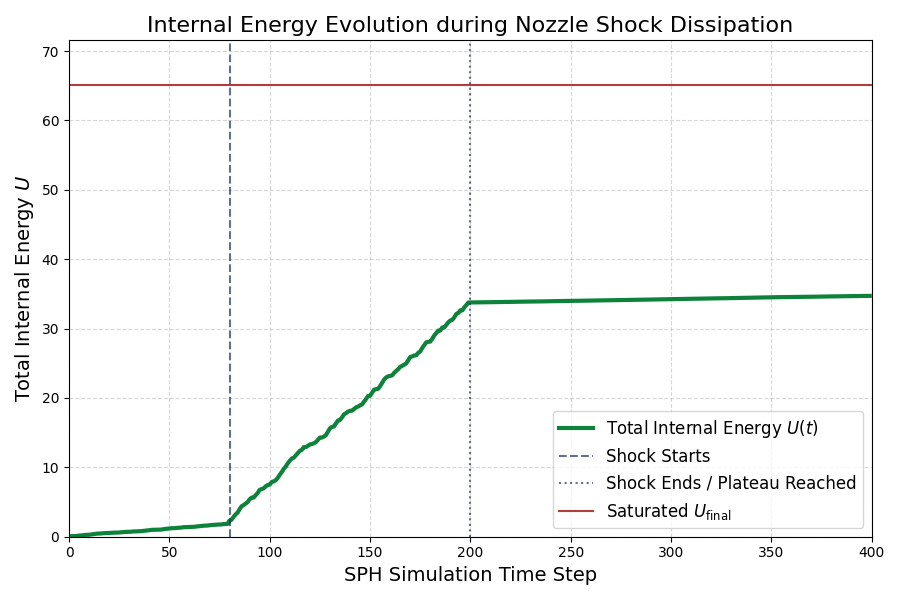
\includegraphics[width=0.6\textwidth]{figure/internal_energy.png}
\caption{Evolution of Total Internal Energy $U(t)$ during Nozzle Shock Dissipation in the TDE accretion stream from \agent. The plot tracks the total internal energy $U(t)$ as a function of SPH time step $\tau$. The shock dissipation phase begins at $\tau \approx 80$ (left) and reaches a saturation plateau ($U_{\text{final}} \approx 34$) at $\tau \approx 200$ (right). The red line marks the theoretical maximum energy ceiling $U_{\text{max}} \approx 65$, confirming that the energy conversion is physically bounded.} 
\label{fig:tde_energy}
\end{figure}

\noindent \textbf{Conclusion}

Semi-analytic PN/Kerr estimates predict moderate misalignment ($\theta \approx 20^\circ$) at $r_p \approx 47 r_g$, with oblique shocks thermalizing $\sim 50\%$ of relative kinetic energy in SPH proxies, consistent with strong shocks dissipating the normal velocity component. Differential precession enhances nozzle dissipation by a factor $\sim 4$ over single-energy baselines, agreeing in order of magnitude across methods.

The traceable workflow yields interpretable results matching initial estimates within 0.5 orders of magnitude. Outputs reproduce expected semi-analytic values under typical parameters, with refined numerical integration and SPH confirming predictions.

Scientifically, the output of \agent validates the hypothesized physics: while differential precession opens an extra dissipation channel, enhancements are less than 1 order of magnitude in typical parameter space. This negative result excludes a competitive hypothesis for resolving TDE energy crises, directing future theory. 

Looking forward, scaling this framework to a broad parameter sweep over black hole mass, spin, orbital inclination, and stellar structure would transform the study of TDE circularization from isolated case analyses into a systematic, semi-automated exploration of dissipation channels across phase space, enabling rapid falsification or validation of competing disk-formation scenarios.

The autonomous derivation, coding, and analysis of \agent is comparable to senior Ph.D in astrophysics, which highlights AI's potential in frontier exploration.

\subsection{Autonomous Discovery: Hamiltonian Construction and Amplitudes Prediction for Semi-leptonic Decays of Charmed Mesons}

%% Background
\noindent \textbf{Background and Motivation}

Semi-leptonic decays of charmed mesons provide a clean environment for studying weak interactions and non-perturbative QCD dynamics. At the quark level, these processes are driven by the charged--current transition
\[
c \rightarrow q\, \ell^+ \nu_\ell , \qquad q=d,s ,
\]
governed by the CKM matrix elements \(V_{cd}\) and \(V_{cs}\). Because the charged lepton and neutrino interact only weakly, the hadronic and leptonic components of the amplitude factorize. As a result, semi-leptonic channels such as
\[
D \to \pi \ell \nu, \qquad D \to K \ell \nu
\]
are ideal probes for extracting heavy--to--light form factors and testing flavor symmetry patterns.

Therefore, constructing the low-energy effective Hamiltonian on hadronic-level, and deriving the amplitudes of these semi-leptonic decays, is essential for understanding symmetry patterns, estimating form-factor relations, and providing controlled predictions relevant for phenomenology and lattice QCD studies.

Although the specific problem studied here has not yet been systematically investigated, closely related studies on the weak decays of singly and doubly charmed baryons have been extensively explored in the literature \cite{Lu:2016ogy,Wang:2017azm,Shi:2017dto}, employing similar symmetry-based and effective-Hamiltonian approaches. Consequently, this well-motivated and timely problem provides a suitable and nontrivial testbed for evaluating the capability of \agent to autonomously explore and solve open problems in theoretical high-energy physics.


\noindent \textbf{Methodology}

From the perspective of flavor SU(3) symmetry, the charmed mesons \(D=(c\bar q)\) form an \(\overline{\mathbf{3}}\) representation, while the light pseudo-scalar mesons reside in the octet \(\mathbf{8}\). The weak current \(\bar q \gamma^\mu (1-\gamma_5) c\) transforms as another \(\overline{\mathbf{3}}\). 

These transformation properties constrain the structure of the effective hadronic Hamiltonian and lead to predictive decay amplitudes in terms of the SU(3) representations.

\medskip
\noindent \textbf{a. Effective Hamiltonian at the Quark Level}

At energies below the \(W\)-boson mass, \agent gives the proper charged-current interaction, which is captured by the four-fermion operator
\[
\mathcal{H}_{\mathrm{eff}}^{\mathrm{(weak)}}
   = \frac{G_F}{\sqrt{2}}\, V_{cq}\,
     \left[ \bar q\, \gamma^\mu(1-\gamma_5) c \right]
     \left[ \bar\ell\, \gamma_\mu(1-\gamma_5) \nu_\ell \right]
     + \text{h.c.},
\]
with \(q=d,s\). Only the hadronic current participates in SU(3) flavor transformations.

\medskip
\noindent \textbf{b. SU(3) Flavor Structure}

\begin{itemize}
    \item The initial charmed meson is represented as: 
    \[D_i = [D^0(c\bar u), D^+(c\bar d), D_s^+(c\bar s)] \in \overline{\mathbf{3}}\]
    \item The weak current is represented as \(O_i =[0,V_{cd},V_{cs}] \in \overline{\mathbf{3}}\).
    \item The final pseudo-scalar meson belongs to the octet \(P^{\,i}_{\; j} \in \mathbf{8}\):
    \[
    P = \begin{pmatrix}
        \dfrac{\pi^0}{\sqrt2}+\dfrac{\eta_8}{\sqrt{6}} & \pi^+ & K^+ \\
        \pi^- & -\dfrac{\pi^0}{\sqrt2}+\dfrac{\eta_8}{\sqrt{6}} & K^0 \\
        K^- & \bar K^0 & -\dfrac{2\eta_8}{\sqrt{6}}
    \end{pmatrix}
    \]
\end{itemize}

Since the octet field is traceless, the most general SU(3)-invariant hadronic Hamiltonian coupling these representations can be written as follows, in which only one independent reduced structure contributes:
\[
\mathcal{H}_{\mathrm{had}}
  \propto  
   a\, P^{\,i}_{\; j}\, O_i\, D^j 
\]
where \(a\) is the SU(3) irreducible amplitude containing the non-perturbative QCD dynamics. 

\medskip
\noindent \textbf{c. Decay Amplitudes Predictions}

For the pseudo-scalar-to-pseudo-scalar transition \(D(p) \to P(p')\), only the hadronic matrix element of the vector current contributes:
\[
\langle P(p')|\bar q \gamma^\mu c|D(p)\rangle
\]
The axial current does not contribute between two pseudo-scalars,
\[
\langle P|\bar q \gamma^\mu\gamma_5 c|D\rangle = 0.
\]
Based on the hadronic Hamiltonian, the full semi-leptonic decay amplitude of charmed meson $D$ is given by
\[
\mathcal{M}(D\to P \ell\nu)
  = \frac{G_F}{\sqrt{2}}\, V_{cq}\,
    \langle P|\bar q \gamma^\mu c|D\rangle
    \left[\bar u_\ell \gamma_\mu (1-\gamma_5) v_{\nu}\right].
\]
From this, the decay amplitudes of all allowed channels can be predicted by \agent, as summarized in Table~\ref{tab:Gamma Matrix Map}.


\begin{table*}[ht]
    \centering
    \renewcommand{\arraystretch}{1.5}
      \setlength{\tabcolsep}{3mm}
    \begin{tabular}{c c}
        \hline\hline
        Decay channels & Amplitudes (in unit of $a$) \\
         \hline
        $D^0\to\pi^-\ell\nu$ & $V_{cd}$   \\

        $D^0\to K^-\ell\nu$ & $V_{cs}$   \\

        $D^+\to\pi^0\ell\nu$ & $-\dfrac{1}{\sqrt2} V_{cd}$   \\
       
        $D^+\to\eta_8\ell\nu$ & $\dfrac{1}{\sqrt6} V_{cd}$   \\
        
        $D^+\to\bar K^0\ell\nu$ & $V_{cs}$   \\

        $D^+_s\to K^0\ell\nu$ & $V_{cd}$   \\

        $D^+_s\to\eta_8\ell\nu$ & $-\dfrac{2}{\sqrt6} V_{cs}$   \\
        \hline
    \end{tabular}
    \caption{SU(3) amplitude predictions for semi-leptonic decays of charmed mesons $D$}  
    \label{tab:Gamma Matrix Map}
\end{table*}

\newpage
\noindent \textbf{Conclusion}

In this work, we demonstrate how \agent can automatically construct the semi-leptonic effective Hamiltonian for charmed meson decays, using both the quark-level weak interaction and the SU(3) flavor structure of the hadronic states.

As a result, \agent successfully determines the correct hadronic-level effective Hamiltonian for the semi-leptonic decays of charmed mesons, and provides physical predictions for the amplitudes of all decay channels. \agent automates a derivation that traditionally requires substantial expertise in weak interactions and flavor symmetry.

Furthermore, this work shows that \agent is capable of constructing effective theoretical models based on physical assumptions and deriving testable physical predictions from them. This highlights \agent’s potential to autonomously explore open problems in physics and to obtain correct physical predictions through self-evaluation.

Looking ahead, extending this autonomous framework to a broader set of heavy-flavor systems and symmetry-breaking patterns would shift such analyses from isolated, hand-crafted derivations to a systematic and reproducible exploration of effective theories, enabling rapid comparison across channels, symmetries, and dynamical assumptions.

\section{Discussion}
\label{sec:dis}

\subsection{Towards Autonomous Scientific Agents}
\label{sec:dis-conclusion}
Current AI scientist systems are still largely optimized for text-centric domains, with limited ability to manipulate rigorous mathematical formalisms and conduct robust numerical computation, while also lacking the adaptability to long-horizon workflows.

More specifically, in physics, a fundamental yet abstract, inherently complex, and intellectually demanding domain, research often requires both intensive analytical reasoning and code-based numerical computation, a dual capability largely absent in previous agents.

To meet the demands of physics research, we propose \agent, an LLM-based agent that can operate as an autonomous theoretical and computational physicist, aiming to liberate talented physicists from tedious engineering tasks and repetitive computations, accelerate the emergence of inspiration and its validation. 

\agent integrates theoretical reasoning and numerical computation techniques. Meanwhile, the exploration methodology of Monte Carlo Tree Search (MCTS) is integrated with hierarchical agent collaboration to balance exploration with efficiency, and adapt to Ultra-long-horizon tasks.

\agent is further equipped with \knowledge, the evolving multi-layered knowledge base constructed to meet the information demands of real scientific research scenarios, enabling more efficient and robust scientific investigations, with a strong emphasis on functionality. Information extracted from retrieved pares, reusable validated reasoning paths, and reliable priors together constitute a representative paradigm for an AI scientist’s knowledge infrastructure. In contrast, other works on scientific knowledge base place greater emphasis on the systematic organization and structural completeness of knowledge, achieving superior coverage but differing in design philosophy from the current LANDAU framework. These approaches are complementary in nature, and their integration represents a promising direction for future exploration.

\newpage
Across scales ranging from the cosmos to fundamental particles, and from elementary interaction laws to the emergence of diverse quantum phases of matter, our \agent has demonstrated reliable capabilities and decent scientific autonomy the validation cases:

\vspace{-1.6ex}
\begin{itemize}
    \item \textbf{Acceleration}: In two typical cases, \agent compresses the labor-intensive engineering parts of genuine physics research into less than 6 hours, which typically requires 1-3 months. We expect \agent to eliminate the barrier to mastering trivial techniques and liberate the talented researchers from tedious, repetitive engineering tasks.
    \item \textbf{Automation}: In two semi-open problems cases with moderate novelty, given a human-specified hypothesis, plan, or selected methods, \agent to automatically execute the exploration loop, running experiments, validating hypotheses, thereby substantially compressing the end-to-end research cycle into 1 day.
    \item \textbf{Autonomous Discovery}: In one typical case, \agent conducts fully independent exploration of a problem a scientific problem that remains open, proposing and verifying an innovative model, marking the transition from AI as a co-pilot to an auto-pilot in scientific research.
\end{itemize}
\vspace{-1.6ex}

\vspace{-2.4ex}
\subsection{Limitations and Future Work}
\label{sec:dis-limitation}
While \agent achieves remarkable autonomy in theoretical and computational physics, it inherits certain limitations from its underlying LLMs. The agent's performance is bounded by the LLM's knowledge cutoff and reasoning depth, particularly in highly abstract areas such as string theory or formal quantum field theory, where pure symbolic manipulations remain challenging compared to code-intensive tasks. Additionally, residual hallucinations in the LLM-based critic can occur during evaluations of novel concepts, potentially introducing biases or overlooking viable paths in open-ended explorations. The reliance on retrieved knowledge also assumes high-quality literature access, which may vary in emerging or niche subfields.

To overcome these challenges and propel the development of reliable autonomous scientific agents, upcoming efforts will emphasize innovative strategies. We intend to embed sophisticated debugging and performance analysis utilities, allowing the system to iteratively refine its computational implementations for optimal resource usage and accuracy. Moreover, introducing an enhanced error-checking framework with automated cross-verification against established benchmarks and anomaly detection algorithms will fortify the system's dependability, reducing the impact of inherent model inaccuracies. To broaden its analytical scope, we aim to fuse \agent with dedicated theorem-proving tools and symbolic computation platforms, thereby augmenting its proficiency in intricate theoretical proofs and derivations while leveraging its current expertise in empirical modeling. In the broader perspective, our vision includes transforming the architecture into an expansive collaborative network of agents adept at tackling multifaceted, cross-domain research endeavors, incorporating mechanisms for ongoing knowledge updates from external data sources and seamless integration with experimental apparatuses. These advancements are geared toward establishing comprehensive AI-orchestrated research pipelines, heralding a new era in AI4Science and expediting progress in core scientific fields.

Looking ahead, a central vision of our work is to transform \textsc{PhysMaster} into a practical and powerful AI scientist product for use by physicists, which will be regarded as our highest-priority objective. At the same time, we place equal attention on extending the boundaries of system capabilities—particularly through the optimization of the \knowledge and its adaptation to a broader range of scientific computing scenarios—so that the system can be rigorously evaluated in increasingly complex scientific settings.

\newpage
\bibliography{main}

\end{document} 
